\chapter{Data Analysis}
As mentioned before, though of fast flipping and tremendous effort to keep 
electron beam in exactly the same conditions (intensity, energy, position 
and angle on target) through opposite helicity states, unfortunately, 
there is no way to achieve such a goal. 
After all, no one can understand completely and control every aspect of
something as complicated as an accelerator. There is always various noise caused
in various parts of the machine, though very small in general sense, they are
large enough compare to what we want to measure, and actually the largest correction
to PV asymmetry. So we need to reduce such noise in the raw asymmetry we measured.

We use the same methods to process both PREX-II and CREX data, therefore we will
discuss only CREX data here, anything that is different in PREX-II will be listed
out.

\begin{table}
    \centering
% with cut ErrorFlag&0xda7e6bff == 0 and minirun_size >= 4500
    \begin{tabular}{c | c}
	\hline
	number of good slugs	    & 121   \\
	number of good runs	    & 1384  \\
	number of good miniruns	    & 8525  \\
	number of good quadruplets  & 86832046  \\
	\hline
	charge asymmetry    & $\sim 100\ ppb$\\
	position difference & $\sim 10\ nm$\\
	angle difference    & $\sim 1\ nrad$\\
	energy difference   & $\sim 10\ ppb$\\
	\hline	    
	raw asymmetry	    & $2087\ ppm$\\
	regressed asymmetry & $2090\ ppm$  \\
	\hline
    \end{tabular}
    \caption{CREX Data Statistics}
\end{table}

\begin{table}
    \centering
    \begin{tabular}{c | c c c}
	\hline
	variable    & regression    & dithering	    & Lagrangian    \\
	\hline
	slope	\\
	correction ($ppm$)  \\
	\hline
    \end{tabular}
\end{table}

\begin{comment}
    % https://prex.jlab.org/DocDB/0000/000009/001/riordan_err_recommend-3.pdf
    \begin{itemize}
	\item (design) PREX-II statistical width: $\sim 120\ ppm @30Hz$
	\item (design) BCM resolution: $40\ ppm$
	\item (measured) 1 MHz BCM electronics: $\sim 25\ ppm @30 Hz, 20\ \mu A$
	\item charge and position jitter
	    $$ A_Q: 100-300\ ppm \quad \Delta x: 5-25\ \mu m$$
    \end{itemize}
\end{comment}

%%%%%%%%%%%%%%%%%%%%%%%%%%%%%%%%%%%%%%%%%%%%%%%%%%%%%%%%%%%%%%%%%%%%%%%%
\section{Raw Data}
CREX started commissioning around December 2019, we took the first good run on 
Dec 12. 6 slugs (slug 100 - 105) were collected before the Christmas break. After 
the Christmas break, data taking was resumed until Jan 18 2020 when the first \Ca 
target was damaged accidentally. It took 5 days to prepare a new \Ca target.
Things moving on quite smoothly, we had 2 days of transverse asymmetry (AT)
measurement from Feb 10 to Feb 12. We were a little over halfway on data taking 
when Covid-19 hit and the lab was shut down at the end of March 2020. Fortunately,
things came back 4 months later, we had the chance to continue data taking for
about 1 month. The experiment stopped data taking on Sep 18 2020. A total charge
of 480 C was collected, among which 390 C was good charge. The dataset is clearly
separated into 3 parts: before AT, after AT (before Covid) and after Covid, in
chronological order. A more reasonable split is to separate them by their wien-flip
states, whose result almost overlaps with the chronological separation.

\begin{figure}[h!]
    \begin{tikzpicture}
	\begin{scope}
	    \node[anchor=south west, inner sep=0] (image) at (0, 0)
	    {   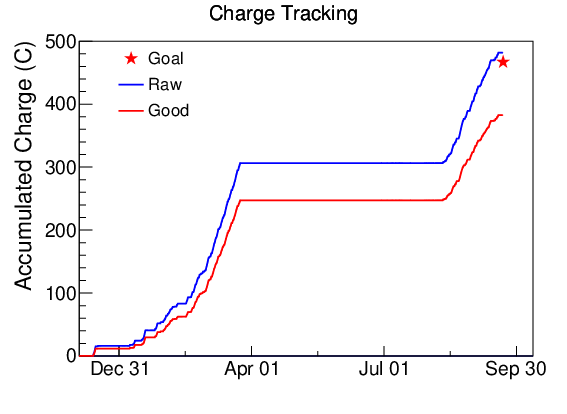
\includegraphics[width=0.45\linewidth]{charge_vs_time}
		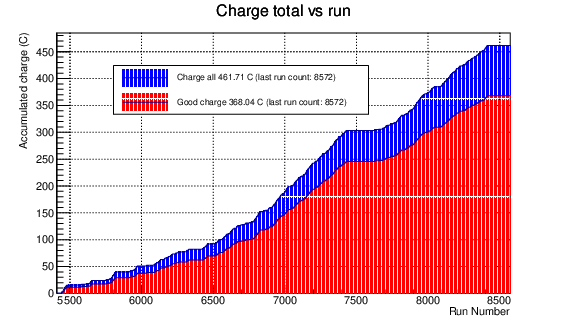
\includegraphics[width=0.55\linewidth]{charge_vs_run} };
	    \begin{scope}[x={(image.south east)},y={(image.north west)}]
		\node [Violet] at (0.27, 0.8) {Covid-shutdown};
		\draw [-stealth, Violet, line width=1pt] (0.28, 0.75) -- (0.28, 0.6);
		\node [Violet] at (0.14, 0.65) {AT};
		\draw [-stealth, Violet, line width=1pt] (0.14, 0.61) -- (0.14, 0.3);
	    \end{scope}
	\end{scope}
    \end{tikzpicture}
    \caption{Charge accumulation versus time (left) and run number (right). The
    long plateau on the left plot is due to Covid shutdown, which is shown around
    run 7500 on the right plot. One sees that data taking was most efficient after
    AT (before Covid), the last month (after Covid) is not bad while the 
    first 2 months is not so efficient due to various problems.}
\end{figure}

CREX collected 1451 production runs, among them, 1386 were identified as `Good'
and used for final analysis. The good runs consists of 1362 both arms runs,
6 left arm runs and 18 right arm runs. Each good production run took about $1\ hour$
and collected about $0.3\ C$ charge with a charge efficiency of 80\%.
\begin{figure}[!h]
    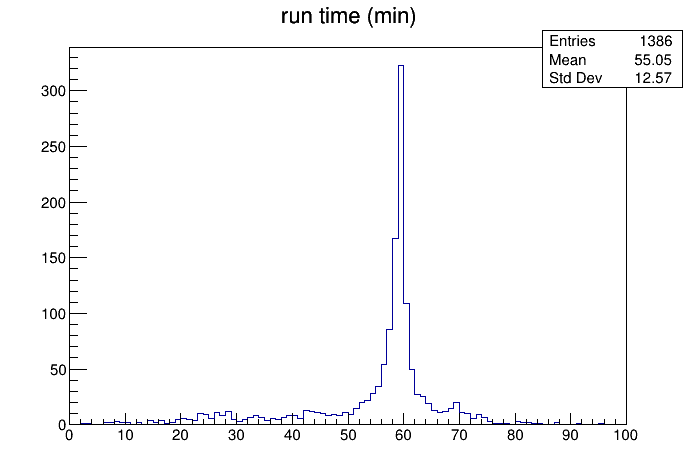
\includegraphics[width=0.32\linewidth]{crex_run_time}
    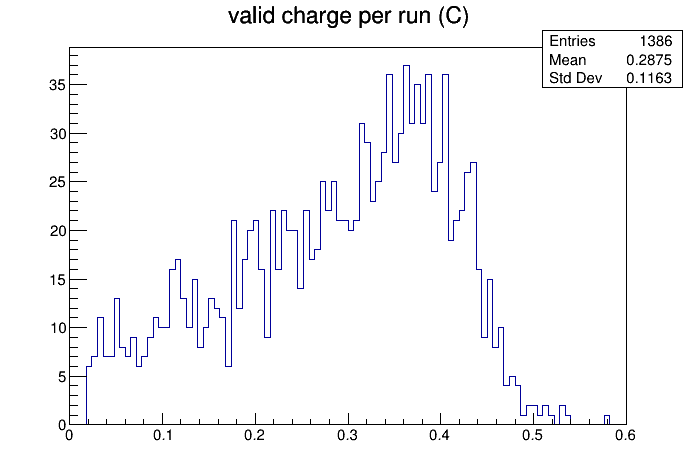
\includegraphics[width=0.32\linewidth]{crex_run_charge}
    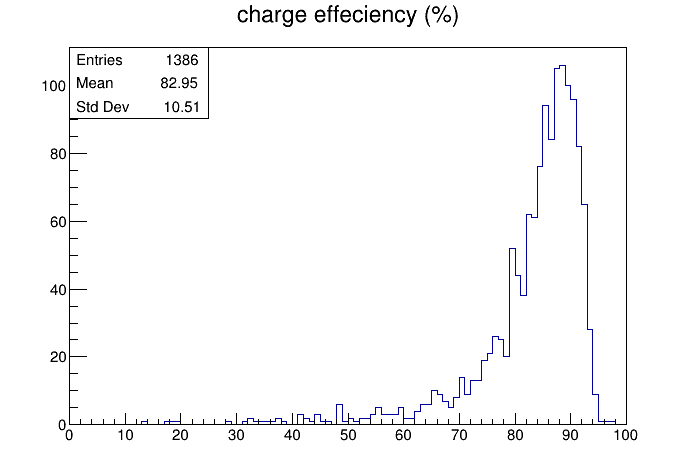
\includegraphics[width=0.32\linewidth]{crex_run_charge_efficiency}
    \caption{Runtime and charge statistics of CREX runs. (\texttt{ErrorFlag == 0})}
\end{figure}

Though electrons came bunch by bunch, the bunch frequency of $499\ MHz$ is much
larger than our helicity flipping frequency of $120\ Hz$, so electron beam can be regarded
as continous. All scattered electrons in one helicity window will be integrated as 1
readout (event). Every 4 continuous helicty windows were grouped into one quadruplet 
(in case of $240\ Hz$ flipping frequency in PREX-II, every 8 helicity windows 
were grouped into one octuplet).
In order to cancel the $60\ Hz$ line power noise, and asymmetry was
calculated based on helicity quadruplet (octuplet in the case of $240\ Hz$), 
whose frequency was $30\ Hz$, as shown in Fig.~\ref{fig:helicity_pattern}. 
CREX collected ??? such good helicity quadruplet.
\begin{figure}[H]
    \centering
    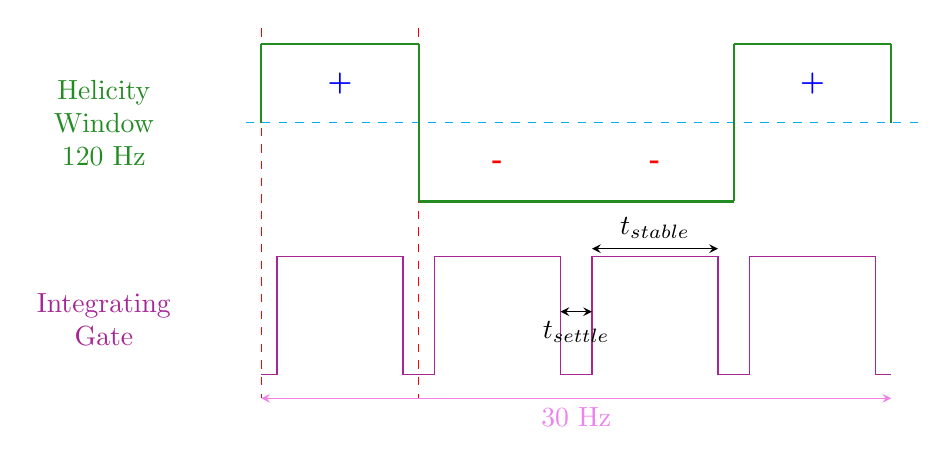
\begin{tikzpicture}[xscale=2]
	\tikzstyle{message} = [align = center]
	\draw[dashed, cyan] (-0.1, 0) -- (4.2, 0);
	\foreach \x in {0, 1}
	{ \draw[dashed, red] (\x, 1.2) -- (\x, -3.5); }
	\foreach \x in {0, 4}
	{ \draw[thick, ForestGreen] (\x, 0) -- (\x, 1); }
	\foreach \x in {1, 3}
	{ \draw[thick, ForestGreen] (\x, -1) -- (\x, 1); }
	\foreach \x in {0, 3}
	{ 
	    \draw[thick, ForestGreen] (\x, 1) -- +(1, 0); 
	    \node[blue] at (\x+0.5, 0.5) {\textbf{+}};
	}
	\foreach \x in {1, 2}
	{ 
	    \draw[thick, ForestGreen] (\x, -1) -- +(1, 0); 
	    \node[red] at (\x+0.5, -0.5) {\textbf{-}};
	}
	\node[message, ForestGreen, very thick] at (-1, 0) {Helicity \\  Window \\ 120 Hz};

	\foreach \x in {0, ..., 3}
	{
	    \draw[Mulberry] (\x, -3.2) -- ++(0.1, 0) -- ++(0, 1.5) -- ++(0.8, 0) 
	    -- ++(0, -1.5) -- ++(0.1, 0);
	}
	\draw[stealth-stealth, black] (2.1, -1.6) -- node[above] {$t_{\text{stable}}$}+(0.8, 0) ;
	\draw[stealth-stealth, black] (1.9, -2.4) -- node[below] {$t_{\text{settle}}$}+(0.2, 0) ;
	\draw[stealth-stealth, Violet] (0, -3.5) -- node[below] {30 Hz} +(4, 0);
	\node[message, Mulberry, very thick] at (-1, -2.5) {Integrating \\ Gate};
    \end{tikzpicture}
    \caption{Schematic plot of Helicity pattern. In CREX, $t_{\text{settle}} = 90\ \mu s$, 
    to allow the PC stablizes after flipping, avoiding any cross effect from last helicity state. 
    The deputy factor is 98.92\%.}
    \label{fig:helicity_pattern}
\end{figure}
\begin{figure}
    \centering
    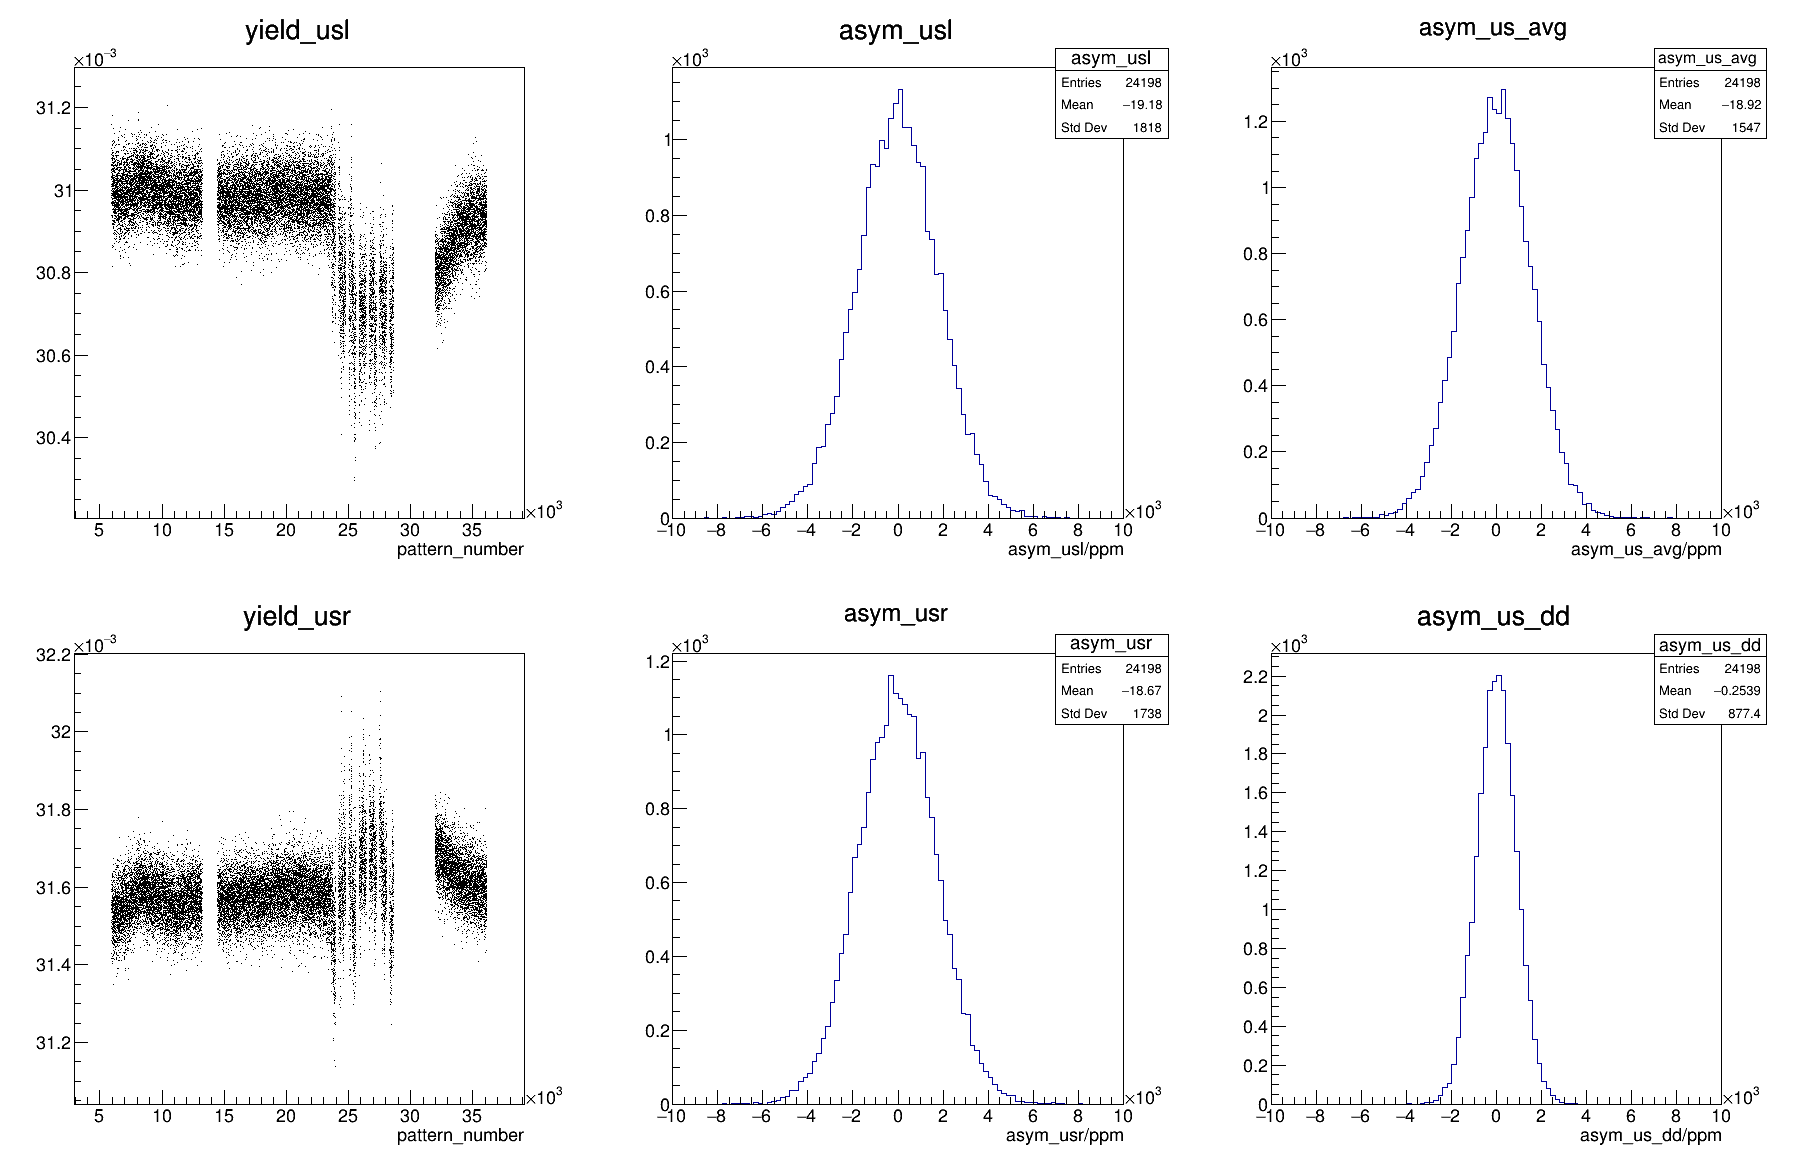
\includegraphics[width=\linewidth]{run_6600_maindet}
    \caption{A run plot: detector yield and asymmetry distribution in run 6600, 
    selected with \texttt{ErrorFlag == 0}. The shift in the second half of the 
    yield plot is caused by beam position/angle fluctuation. 
    The right 2 plots are average and difference of LHRS and RHRS. 
    Ideally, the difference should be 0 and the average is what we want to measure.
    }
\end{figure}

Every run is separated into multiple miniruns to account for the fact that beam
conditions is changing quickly, it is inappropriate to calculate detectors'
response to beam fluctuations -- the detector slope, over a 60 mins time scale. 
Minirun will be more proper, the beam conditions, and therefore
the slope value should be more stable during such a shorter time period.  
Every minirun contains 9000 good (passing cut) quadruplets, which counts about 5~mins
in data taking, the last minirun in each run contains 
whatever number of good quadruplets left that can't be divided into 2 miniruns. 
Miniruns whose number of samples is less half of the standard (4500) will be discarded.
CREX has 8543 miniruns from 1386 good runs, among them, 2 miniruns are discarded
because of small size and 16 miniruns are discarded due to noisy beam conditions 
or large beam shifts that were not caught in the previous 2 respins.
To avoid any respin, these miniruns are simply removed. % which counts ??? C.
\begin{table}
    \centering
    \begin{tabular}{c c c}
	\hline
	run & minirun	& number of samples \\
	\hline
	% 5972	& 0 & 4385  \\
	% 6691	& 0 & 4080  \\
	7720	& 0 & 4352  \\
	8082	& 0 & 4391  \\
	\hline
    \end{tabular}
    \caption{2 Miniruns that have too small good samples. (with cut \texttt{ErrorFlag == 0})}
    \label{tab:short_miniruns}
\end{table}
\begin{table}
% http://ace.phys.virginia.edu/HAPPEX/4606
    \centering
    \begin{tabular}{c c | c c}
	\hline
	run & minirun	& run	& minirun   \\
	\hline
	6564	& 4	& 7211	& 4 \\
	6567	& 2, 4	& 7889	& 0 \\
	6571	& 3, 4	& 7942	& 5 \\
	6593	& 2	& 8036	& 2 \\
	6983	& 8	& 8240	& 1 \\
	7149	& 6	& 8549	& 0, 1, 4   \\
	\hline
    \end{tabular}
    \caption{List of Miniruns that had larger asymmetry outliers and therefore
    were removed.}
\end{table}
\begin{figure}
    \centering
    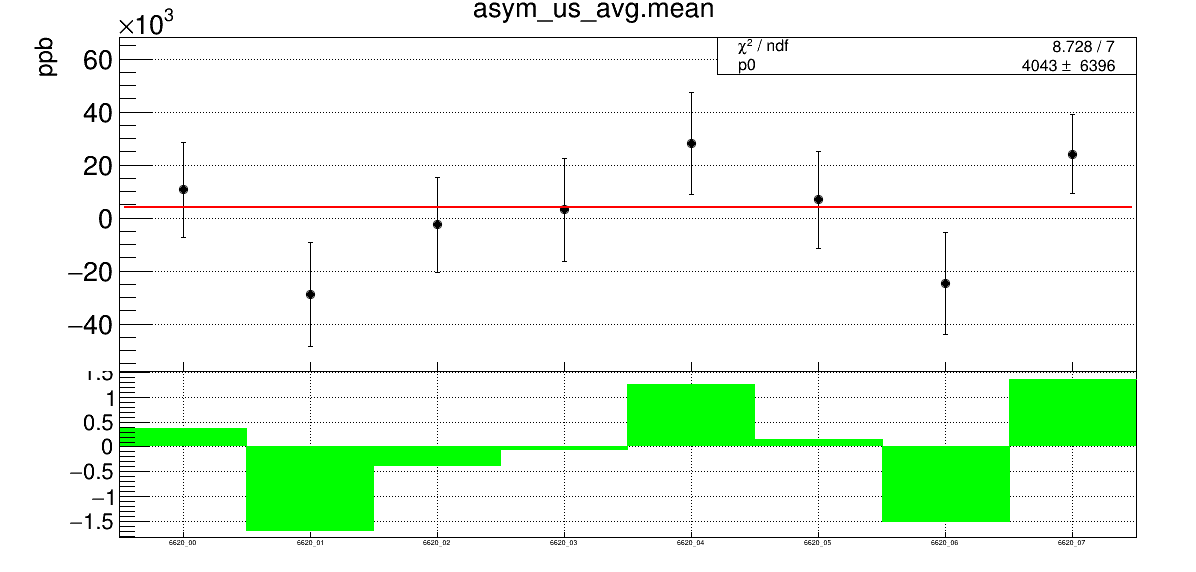
\includegraphics[width=\linewidth]{run_6620_mini_asym_us_avg.mean}
    \caption{A minirun plot: mean values of asym\_us\_avg of each minirun in 
    run 6620 (\texttt{ErrorFlag == 0}).
    The red line is a zero-order polynomial fit and the bottom histogram is
    the ratio of deviation to the mean fit value w.r.t. each point's uncertainty.
    }
\end{figure}

Runs will be grouped into slugs. One slug was defined as all runs between 2
changes of IHWP. With stable beam, we could collect 3 slugs per day, so 
each slug took about 8 hours or longer in case of any accidents. CREX collected
124 slugs, after data cleaning and combination to remove slugs with only 1 run, 
121 slugs were kept.
% slug 100 - 223
% slug 105, 117 and 123 are removed
\begin{figure}
    \centering
    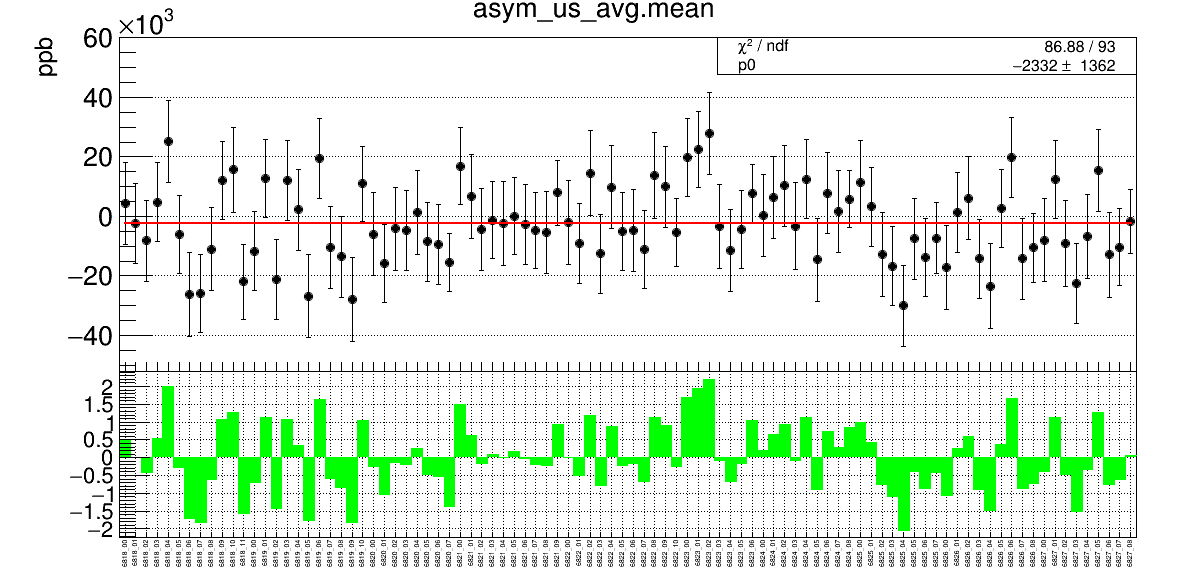
\includegraphics[width=\linewidth]{slug_150_asym_us_avg.mean}
    \caption{A slug plot: minirun-wise distribution of asym\_us\_avg in slug 150 
    (\texttt{ErrorFlag == 0}).}
\end{figure}

Finally, slugs were split into parts, with different wien flip states. We
have 3 parts as said before.
\begin{table}[!h]
    \centering
    \begin{tabular}{c | c}
	\hline
	wien-flip   & slugs \\
	\hline
	right	& 100-137   \\
	left	& 138-185   \\
	right	& 186-223   \\
	\hline
    \end{tabular}
\end{table}

%%%%%%%%%%%%%%%%%%%%%%%%%%%%%%%%%%%%%%%%%%%%%%%%
\subsection{Cut}
A loose cut was applied in the event level to select as much as possible good events.
During data taking, the JAPAN analyzer will check various hardware failures, the
beam stability level, helicity information and others. Based on these 23 checks,
an error code (ErrorFlag), which was the bit-wise OR of the result against each
check, was assigned to each event, an event that passed every check will have
a null error code (ErrorFlag == 0). 

The various hardware failure checks detected the ADC readout in the detectors and
monitors, making sure we were not recording saturation or null values; the 
sample size was also verified. These checks helped to identify the problematic
hardware channels in case of any hardware failures.

The beam stability level checks kept track of beam conditions based on their
mean and RMS values. These checks compared the detectors/monitors readout to 
a user-set upper and lower limit to filter out outliers; besides, for some ADC 
channels, there were cuts on the RMS of a moving time window of 200 (configurable) % prex_ring_stability.xxxx.conf
consecutive events, 
if the RMS value was too large, all events in the time window failed the RMS check. 
Finally, the burplevel check compared current event readout with the average
value of previous 10 (configurable) events, events with difference larger than
the burplevel cut fail this check. With these checks, we can make sure the good 
quality of the data we collected.

One example of such stability cut is the beam current cut. In cases of beam trip
due to various accidents, the beam dropped and then recovered quickly, beam in
the process of falling and rising was usually unstable, so we required the event
beam current should be larger than the stable beam current minus $30\ \mu$A ($15\ \mu$A in PREX-II).

\begin{figure}[!h]
    \centering
    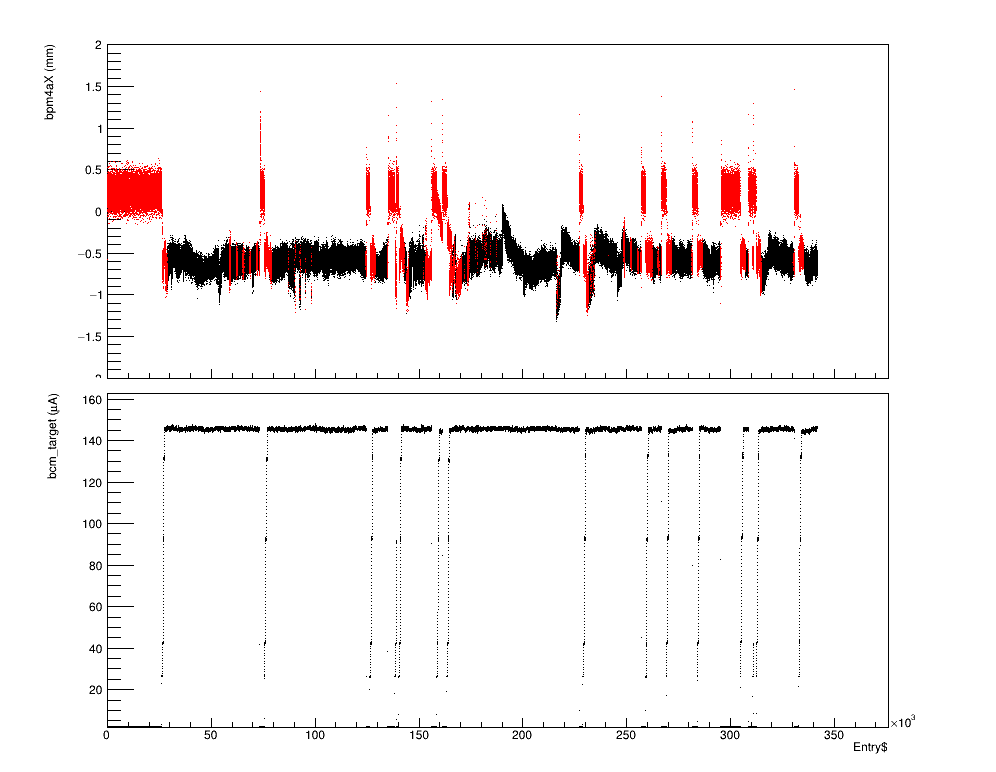
\includegraphics[width=\linewidth]{8019_bpm4aX}
    % 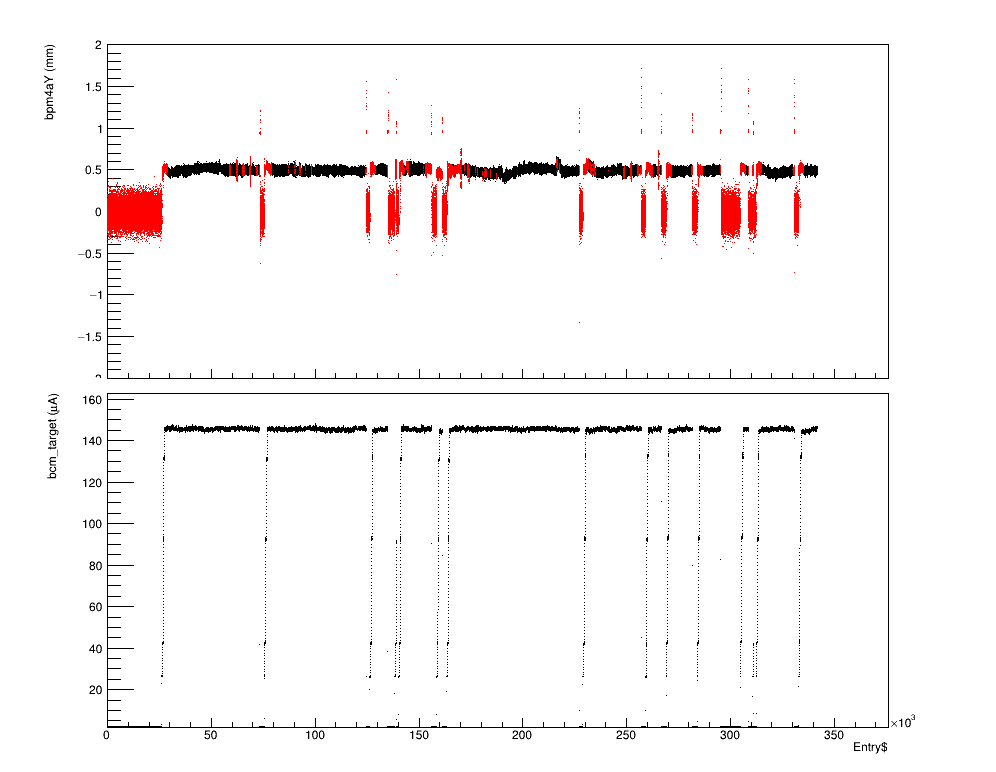
\includegraphics[scale=0.28]{8019_bpm4aY}
    \caption{Bpm4aX distribution in run 8019. Black points are good
    events (\texttt{ErrorFlag == 0}) and red points are bad ones (\texttt{ErrorFlag != 0}). 
    One can clearly see that all beam trips and most beam jitters are recognized 
    by our stability checks.}
\end{figure}

Apart from these checks, we had an analysis shift worker to check monitors/detectors 
yield and their differences/asymmetries for each run after prompting. Additional
cuts can be applied if large beam excursion, drift or any other anomalies were observed. 
These cuts were run specific, added one by one when needed.

During the online and the 2 offline analysis, we used cut \verb|ErrorFlag == 0|
to select good quadruplets, which excluded all beam modulation events. Actually, 
some beam modulation events are usable for our asymmetry analysis and were 
included in our final published result, which counts for about 5\% of the CREX dataset.
To keep consistent with published result, all following plots are produced with cut 
\verb|ErrorFlag&0xda7e6bff == 0|. 

%%%%%%%%%%%%%%%%%%%%%%%%%%%%%%%%%%%%%%%%%%%%%%%%
\subsection{Beam Conditions}
As explained before, the key to measure a teeny tiny asymmetry value is to 
keep all experimental conditions as the same as possible between different 
helicity windows. Among all the conditions that needed precise control, the 
hardest one was beam condition, any fluctuation in any components along the 
long accelerator line will cause changes to beam, therefore introducing false 
asymmetry to our measurement. Though of the difficulties, CEBAF staff worked 
hard to provide us excellent beam with tiny difference between different helicity 
windows, as displayed below.

%%%%%%%%%%%%%%%%%%%%%%%%
\subsubsection{Beam Current}
The raw asymmetry we measured was normalized to the beam current, because beam
current varied from run to run, and even within a single run, beam current was 
slightly different between helicity windows. The normalized raw asymmetry is:
\begin{equation}
    \CA_{raw} = \frac{(D/I)^+ - (D/I)^-}{(D/I)^+ + (D/I)^-}
	\approx \frac{D^+ - D^-}{D^+ + D^-} - \frac{I^+ - I^-}{I^+ + I^-}
	= \CA_D - \CA_I
\end{equation}

We see that the charge asymmetry contributes to our raw asymmetry directly, so
tremendous effort was invested to keep the charge asymmetry as small as possible.
Specifically, this was done through the charge feedback system. Overall, charge
asymmetry was about hundreds of ppb. We can also tell from Fig.~\ref{fig:crex_bcm_target}
that part 2 has relatively good beam conditions than the other 2 parts.
\begin{figure}[H]
    \centering
    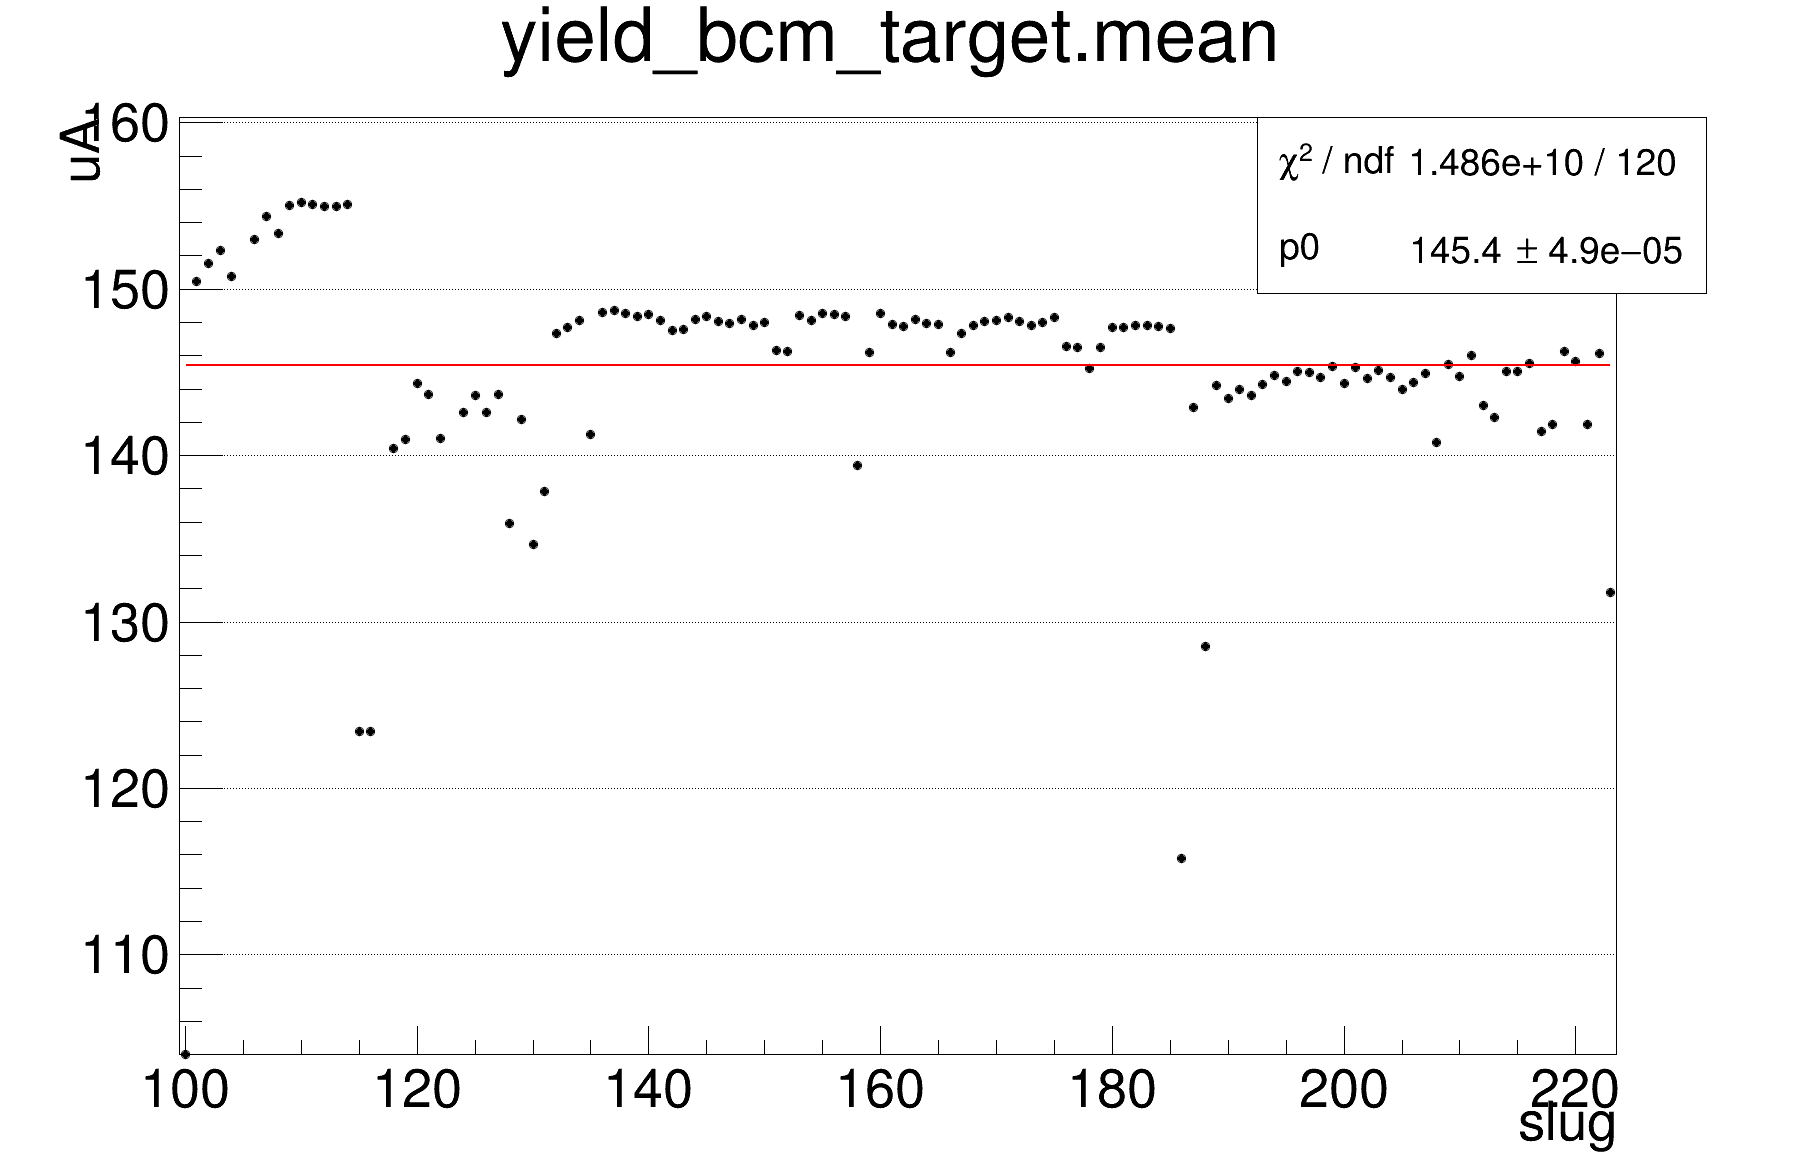
\includegraphics[width=0.32\linewidth]{crex_yield_bcm_target.mean}
    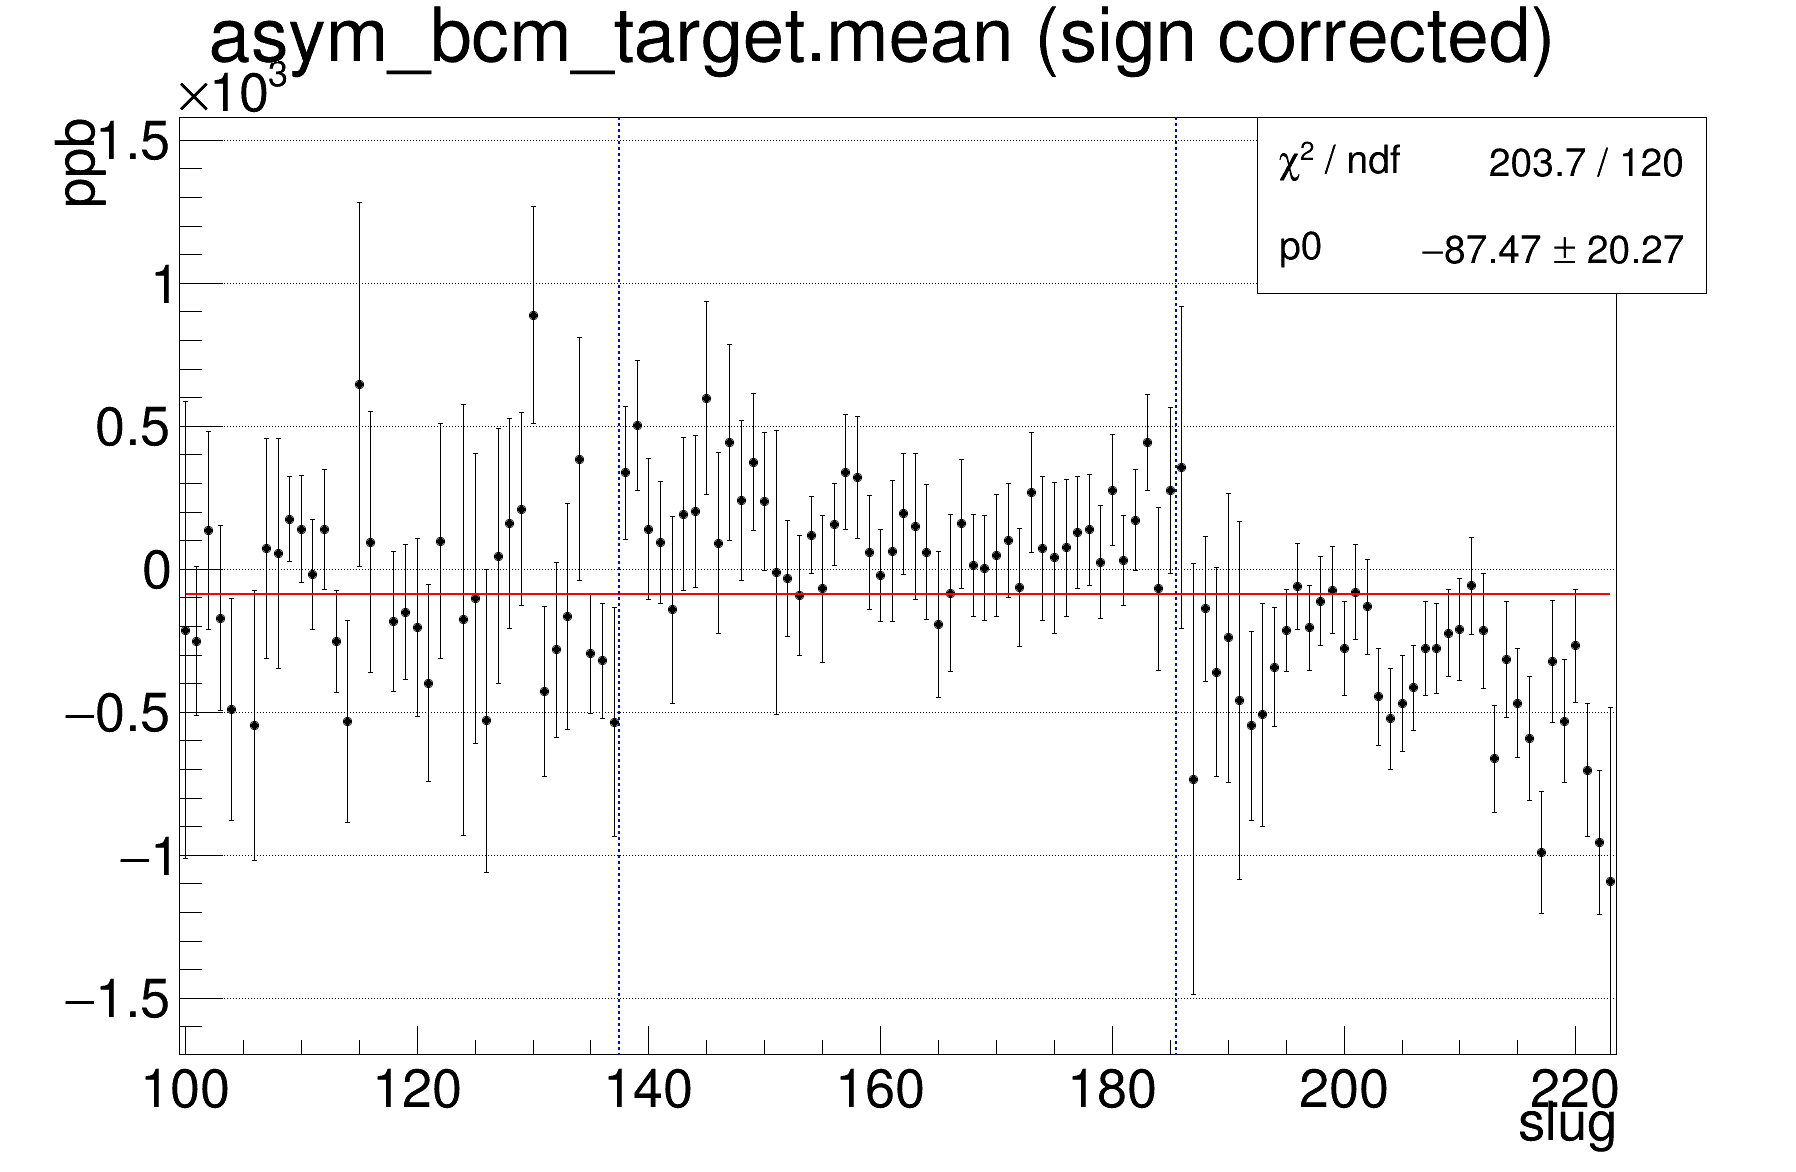
\includegraphics[width=0.32\linewidth]{crex_asym_bcm_target.mean}
    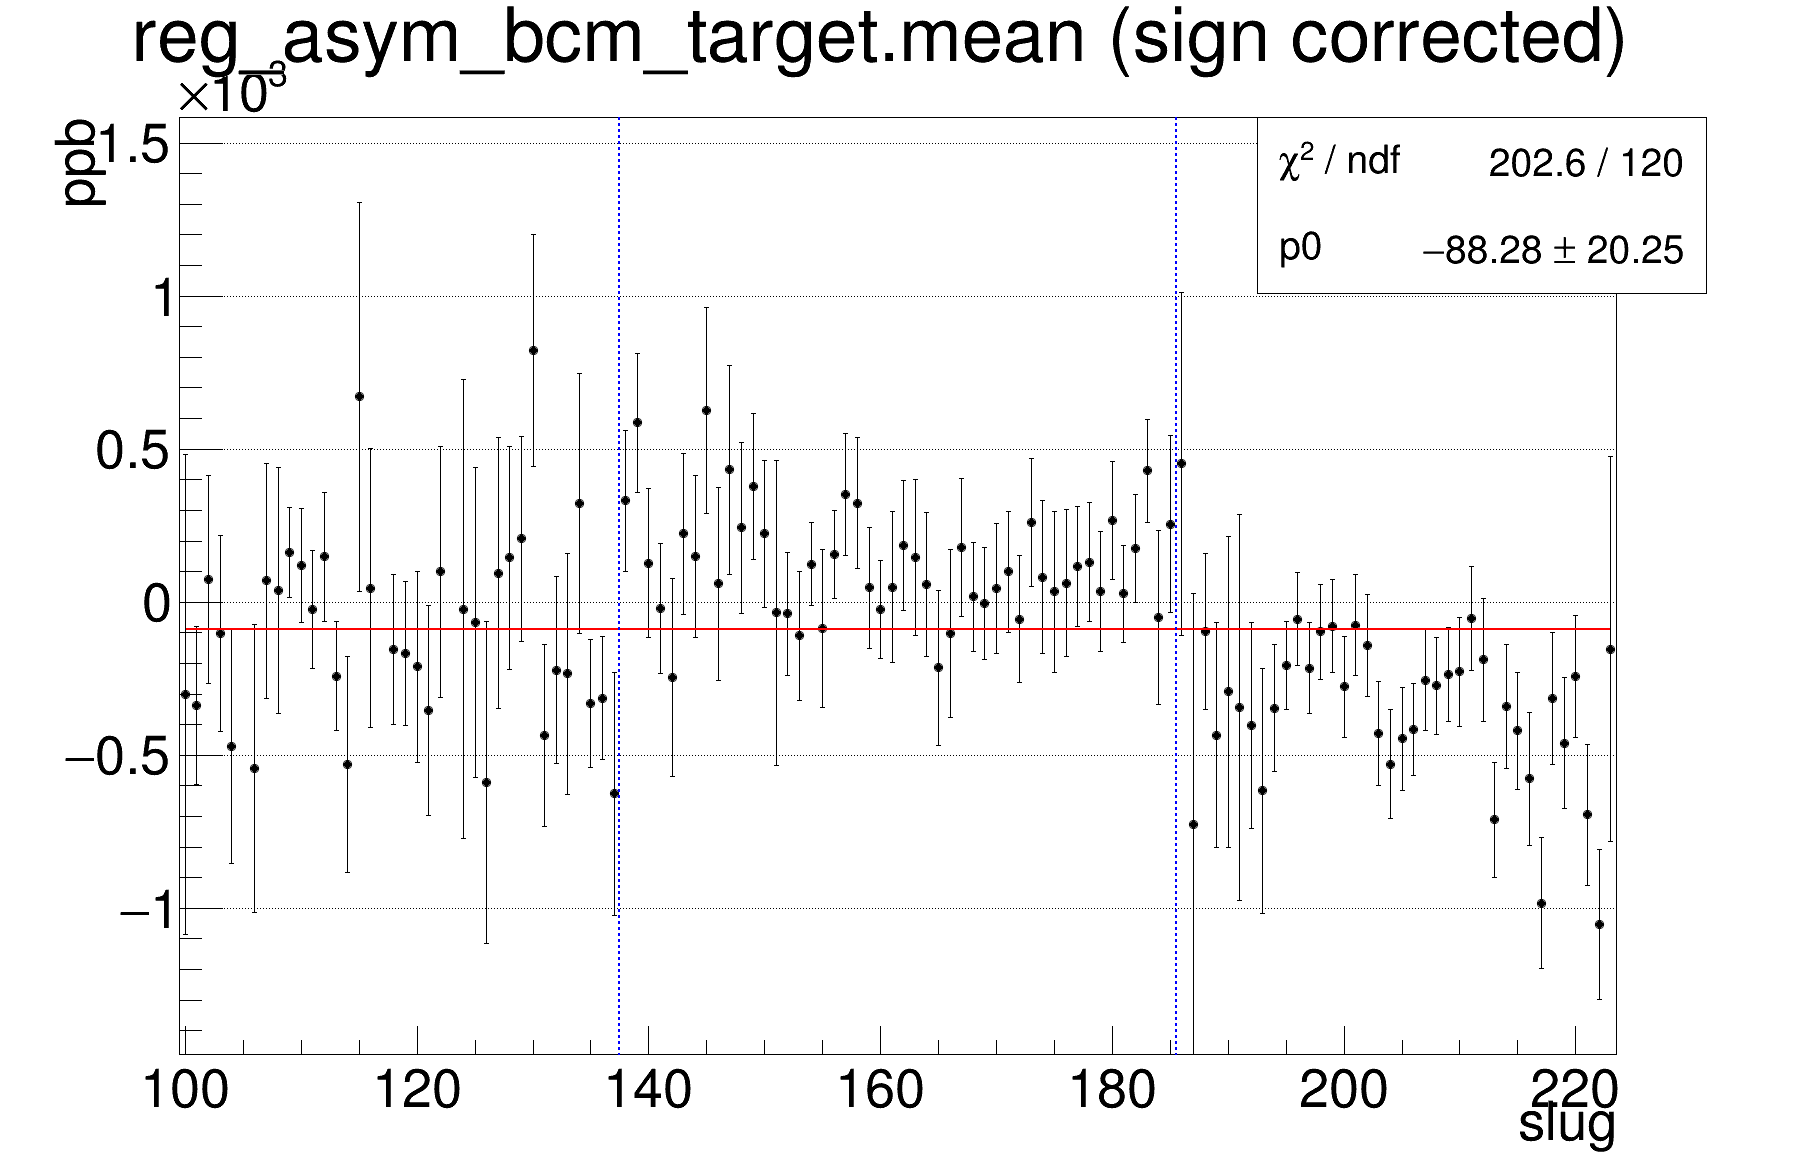
\includegraphics[width=0.32\linewidth]{crex_reg_asym_bcm_target.mean}
    \caption{Slug-wise mean value of beam current yield, asymmetry and regressed 
    asymmetry in CREX (\texttt{ErrorFlag == 0}). The blue dashed lines separate
    the dataset into 3 parts with different wien-flip states.
    Most of the time, CREX run at $\sim 150\ \mu A$, an overall $\sim 100\ ppb$ charge 
    asymmetry was achieved.}
    \label{fig:crex_bcm_target}
\end{figure}

%%%%%%%%%%%%%%%%%%%%%%%%
\subsubsection{Beam Position, Angle and Energy}
% target position/angle oscillation: http://ace.phys.virginia.edu/HAPPEX/4520
We don't have direct measurement of beam position and angle on the target, these 
information can be inferred from various BPMs measurements, though. Given the 
distance between the target and BPM4A as $D1 = 5.725\ m$ and the distance
between BPM4A and BPM4E as $D2 =4.083\ m$, beam position and angle on target 
will be:
\begin{equation}
    \begin{aligned}
	T_{x,y} &= \text{BPM4A}_{x,y} + \frac{\text{BPM4E}_{x,y} - \text{BPM4A}_{x,y}}{D2} D1	\\
	\theta_{x,y} &= \frac{\text{BPM4E}_{x,y} - \text{BPM4A}_{x,y}}{D2} \\
    \end{aligned}
\end{equation}
Using this formula, we get an overall difference of beam position/angle on target as:
\begin{equation*}
    \text{diff}_{X,Y} \sim 10\ nm	\qquad \text{diff}_{\theta_{X,Y}} \sim nrad	
\end{equation*}
Again, the second part has more stable beam than the other 2 parts.

\begin{figure}[H]
    \centering
    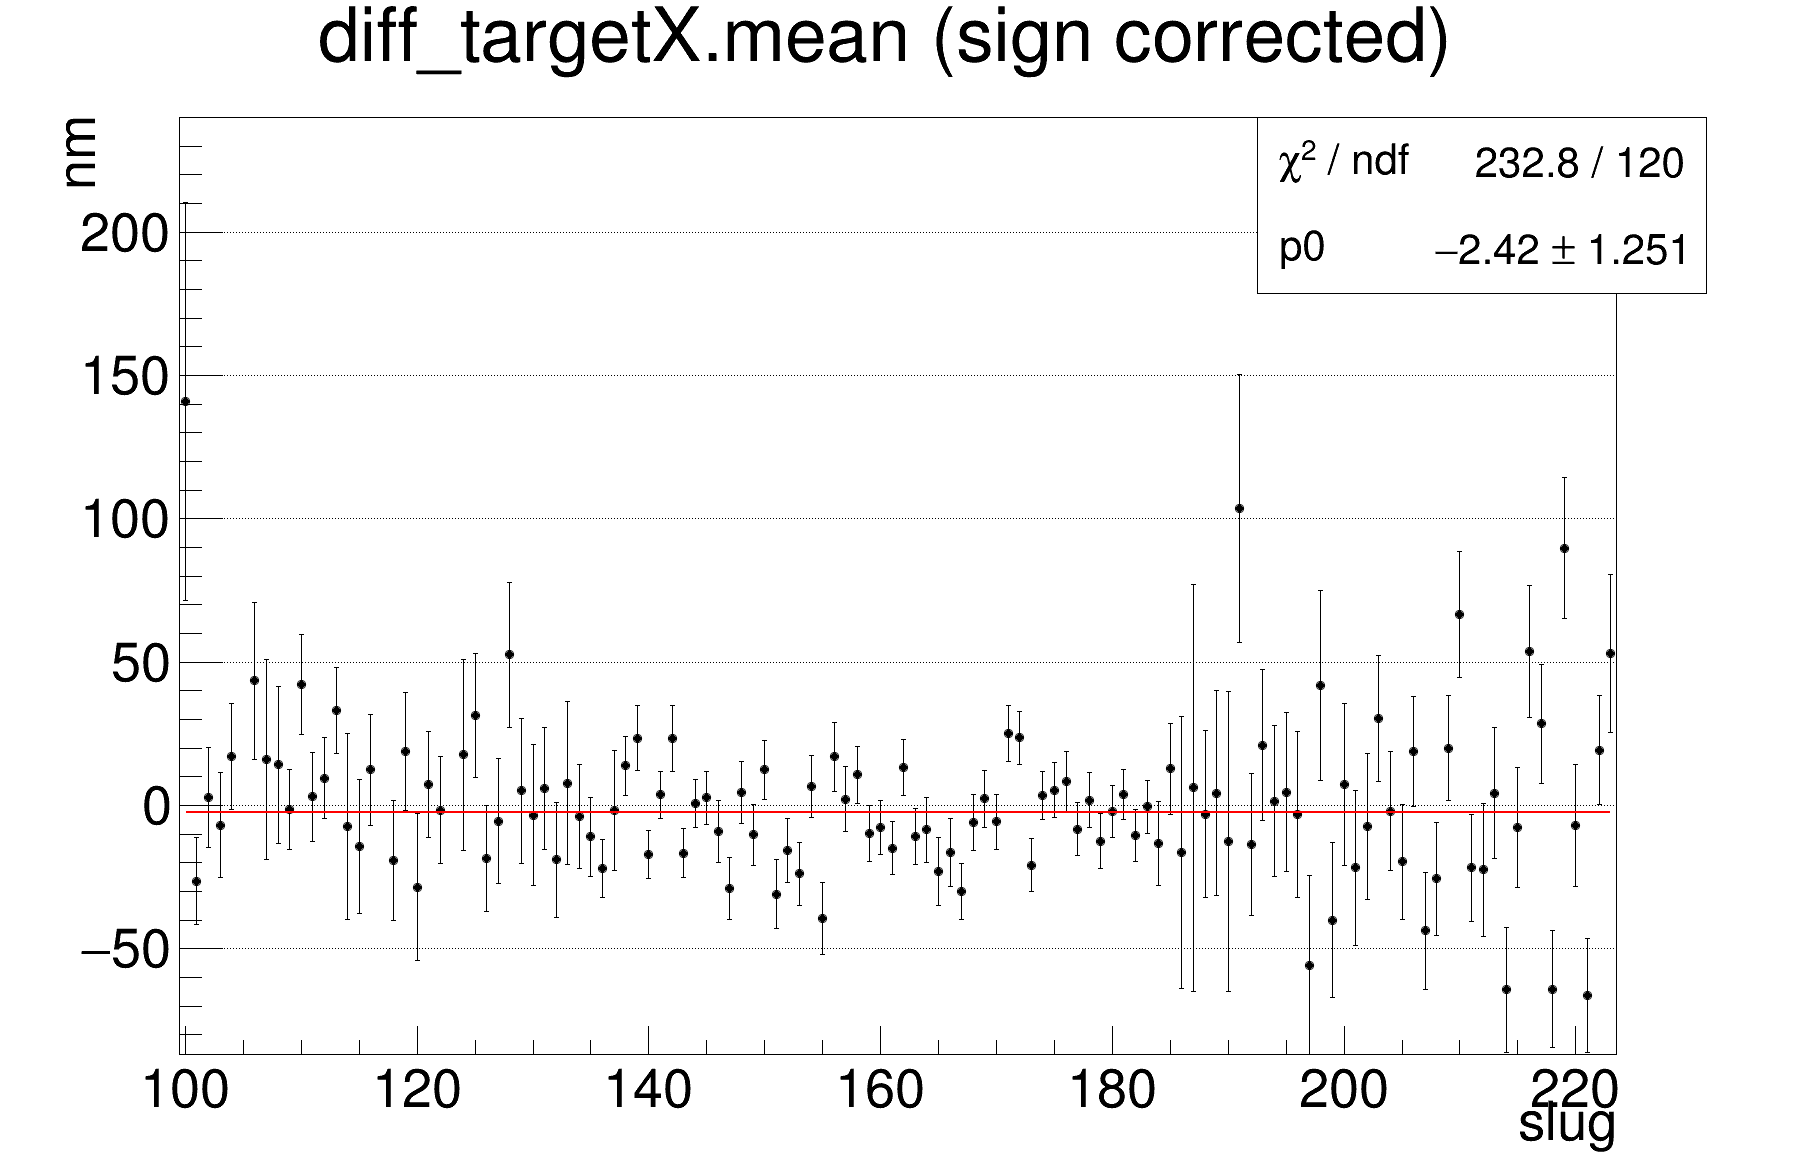
\includegraphics[width=0.49\linewidth]{crex_diff_targetX.mean}
    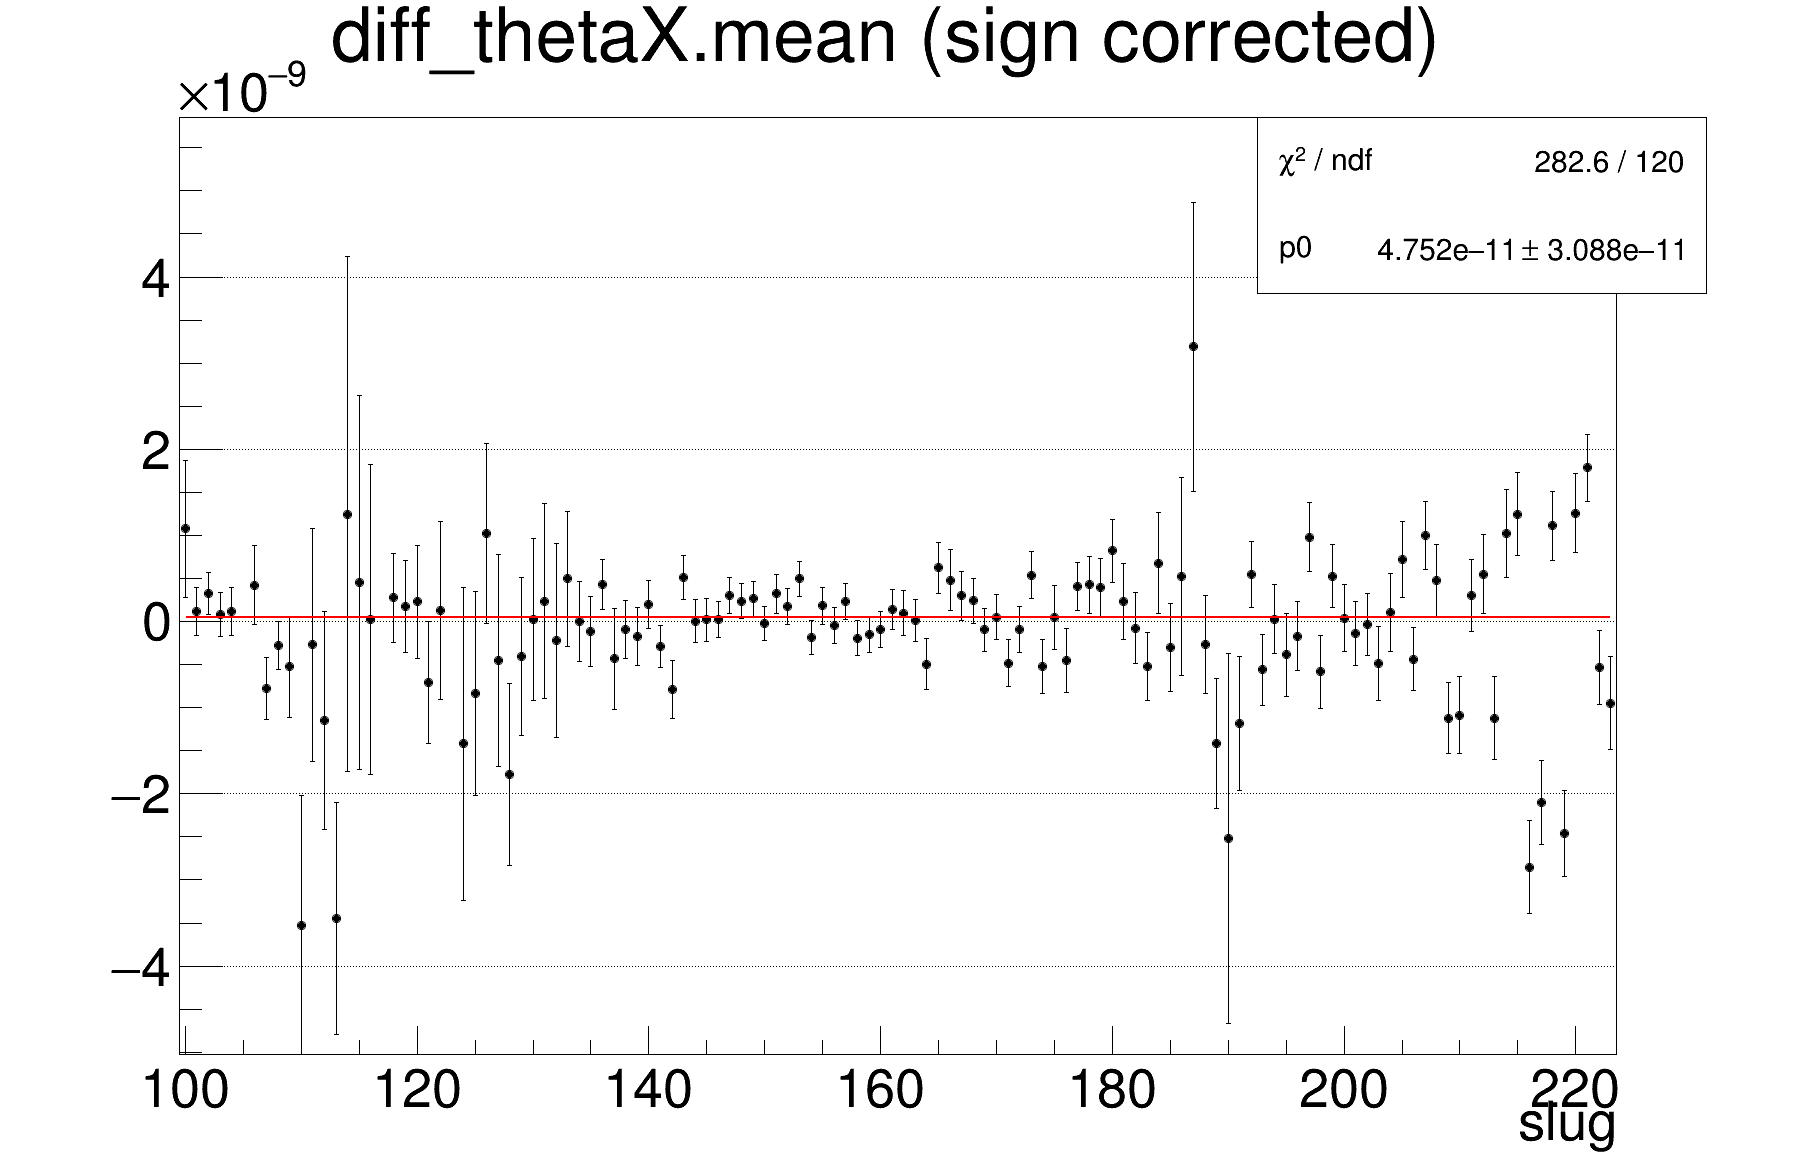
\includegraphics[width=0.49\linewidth]{crex_diff_thetaX.mean}
    \caption{Slug-wise mean value of beam position/angle difference on target. 
    Very precise control of beam conditions was achieved as told by the plot.
    The Y dimension plots are similar and are not shown here.}
\end{figure}


The beam momentum/energy was measured by BPM12X, whose dispersion tells deviation
(dp) from the standard value (p0). The design value of dispersion for CREX was
$D = 4.0\ m$, and an actual measurement gave $\sim3.8$~m. I used 4.0~m here.
As can be seen in Fig.~\ref{fig:crex_diff_p}, CEBAF provided a beam with energy 
dispersion as small as $\sim10\ ppb$.

\begin{equation}
    \frac{dp}{p} = \frac{\text{diff\_bpm12X}}{D}
\end{equation}

\begin{figure}[H]
    \centering
    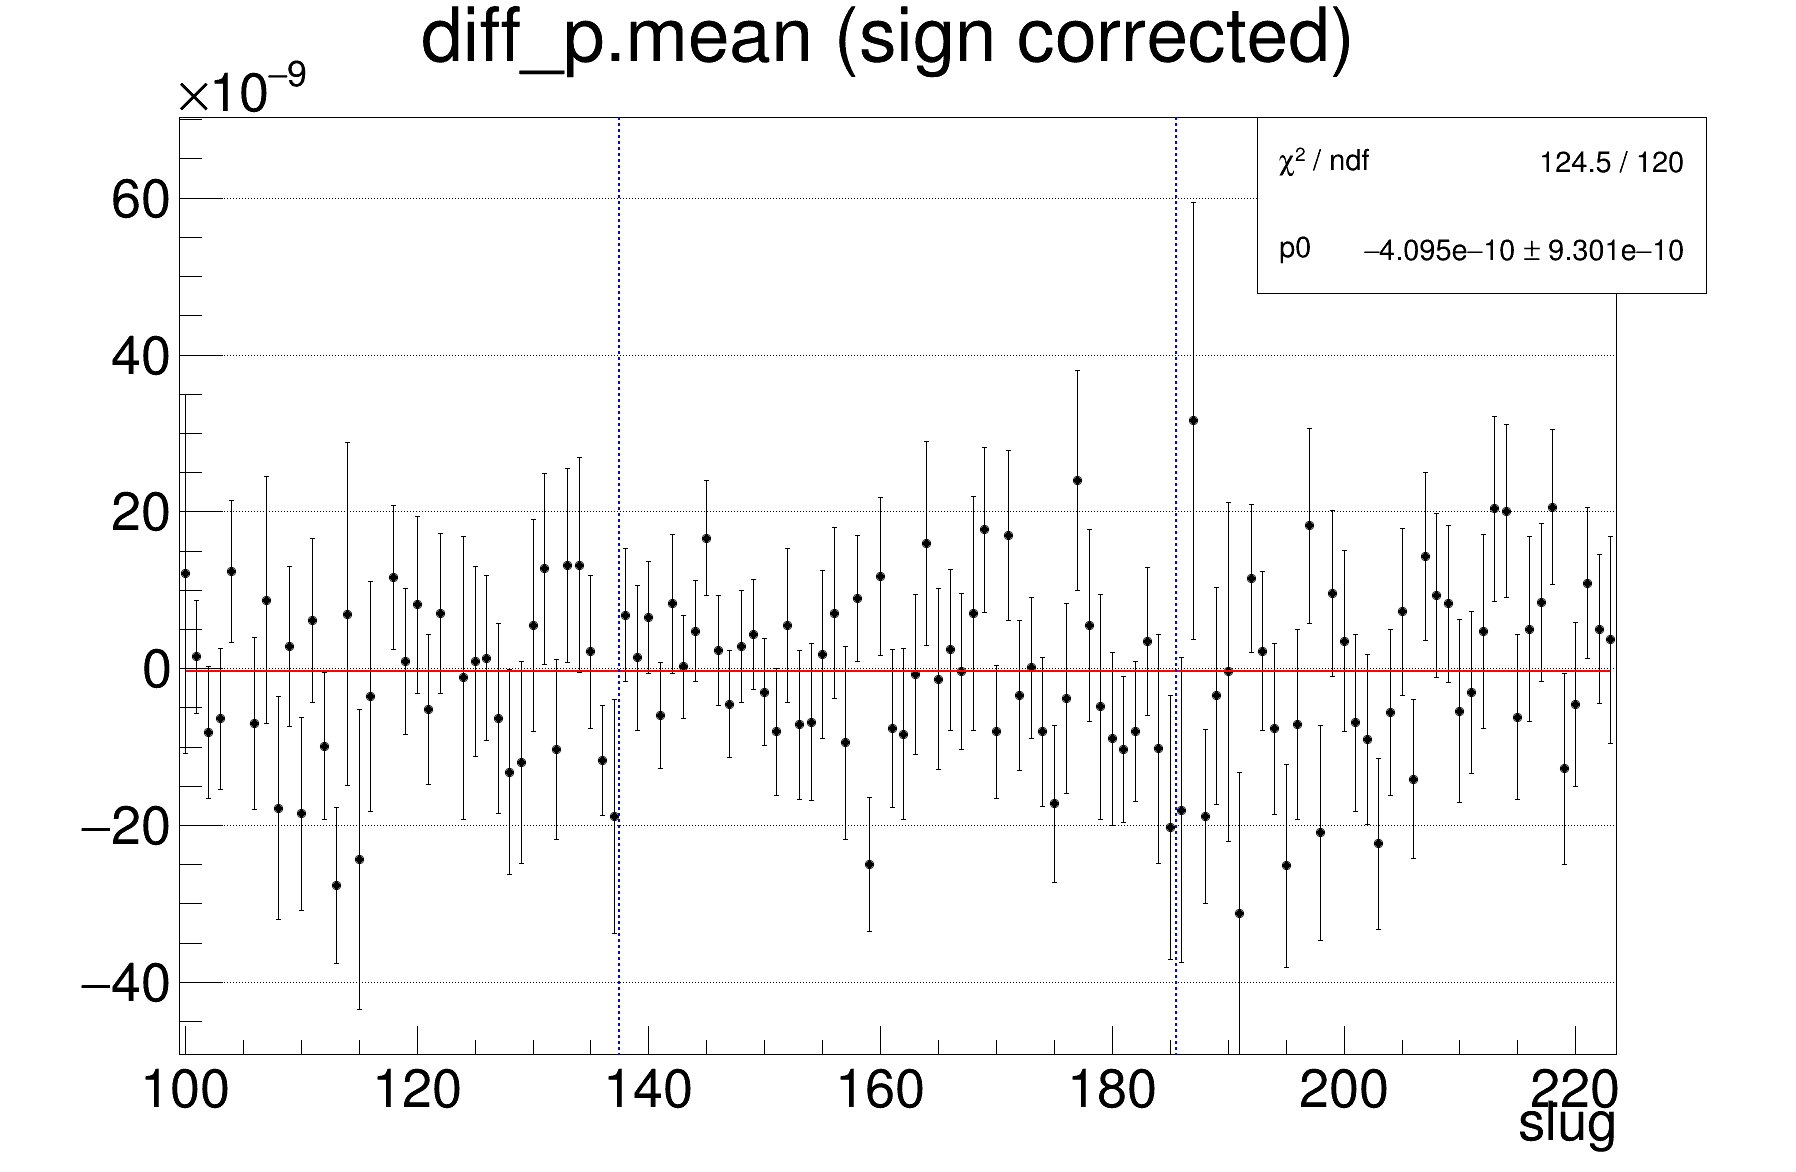
\includegraphics[width=0.6\linewidth]{crex_diff_p.mean}
    \caption{Slug-wise mean value of beam energy dispersion. Overall, $\sim 10$~ppb 
    energy difference was achieved. }
    \label{fig:crex_diff_p}
\end{figure}

%%%%%%%%%%%%%%%%%%%%%%%%%%%%%%%%%%%%%%%%%%%%%%%%
\subsection{Raw Asymmetry}
% pedestal correction
The raw asymmetry is defined as:
\begin{equation}
    \CA_{raw} \equiv 
    \begin{cases}
	\frac{d^+ - d^- - d^- + d^+}{d^+ + d^- + d^- + d^+}	& (+--+\ \text{pattern})    \\
	\frac{-d^- + d^+ + d^+ - d^-}{d^+ + d^- + d^- + d^+}	& (-++-\ \text{pattern})    \\
    \end{cases}
\end{equation}
where $d=\frac{D}{I}$ is the normalized detector integrating yield in one helicity
window, the upper-script indicate helicity of the beam. The detector yield was
calibrated with corresponding pedestals. 
% The raw asymmetry was blinded before final result was freezed.
\begin{figure}[H]
    \centering
    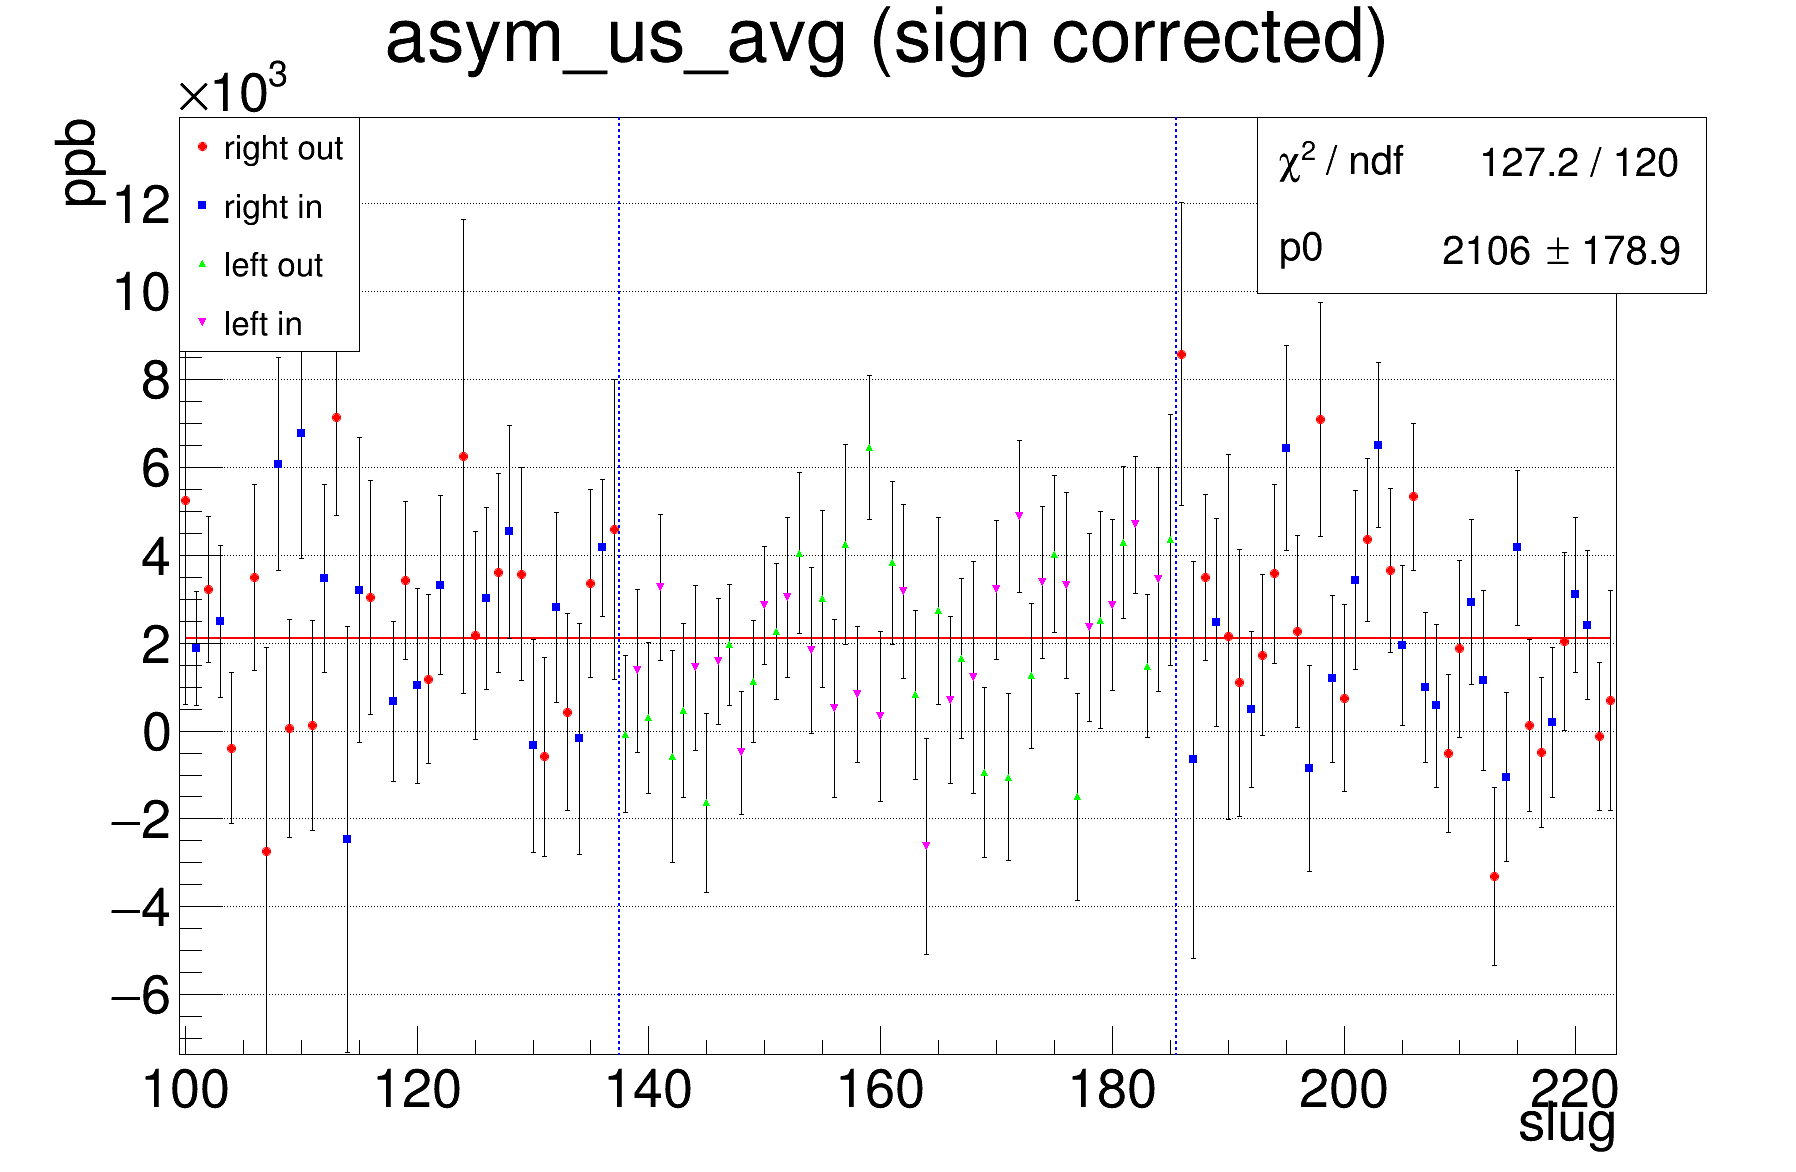
\includegraphics[width=0.49\linewidth]{crex_asym_us_avg}
    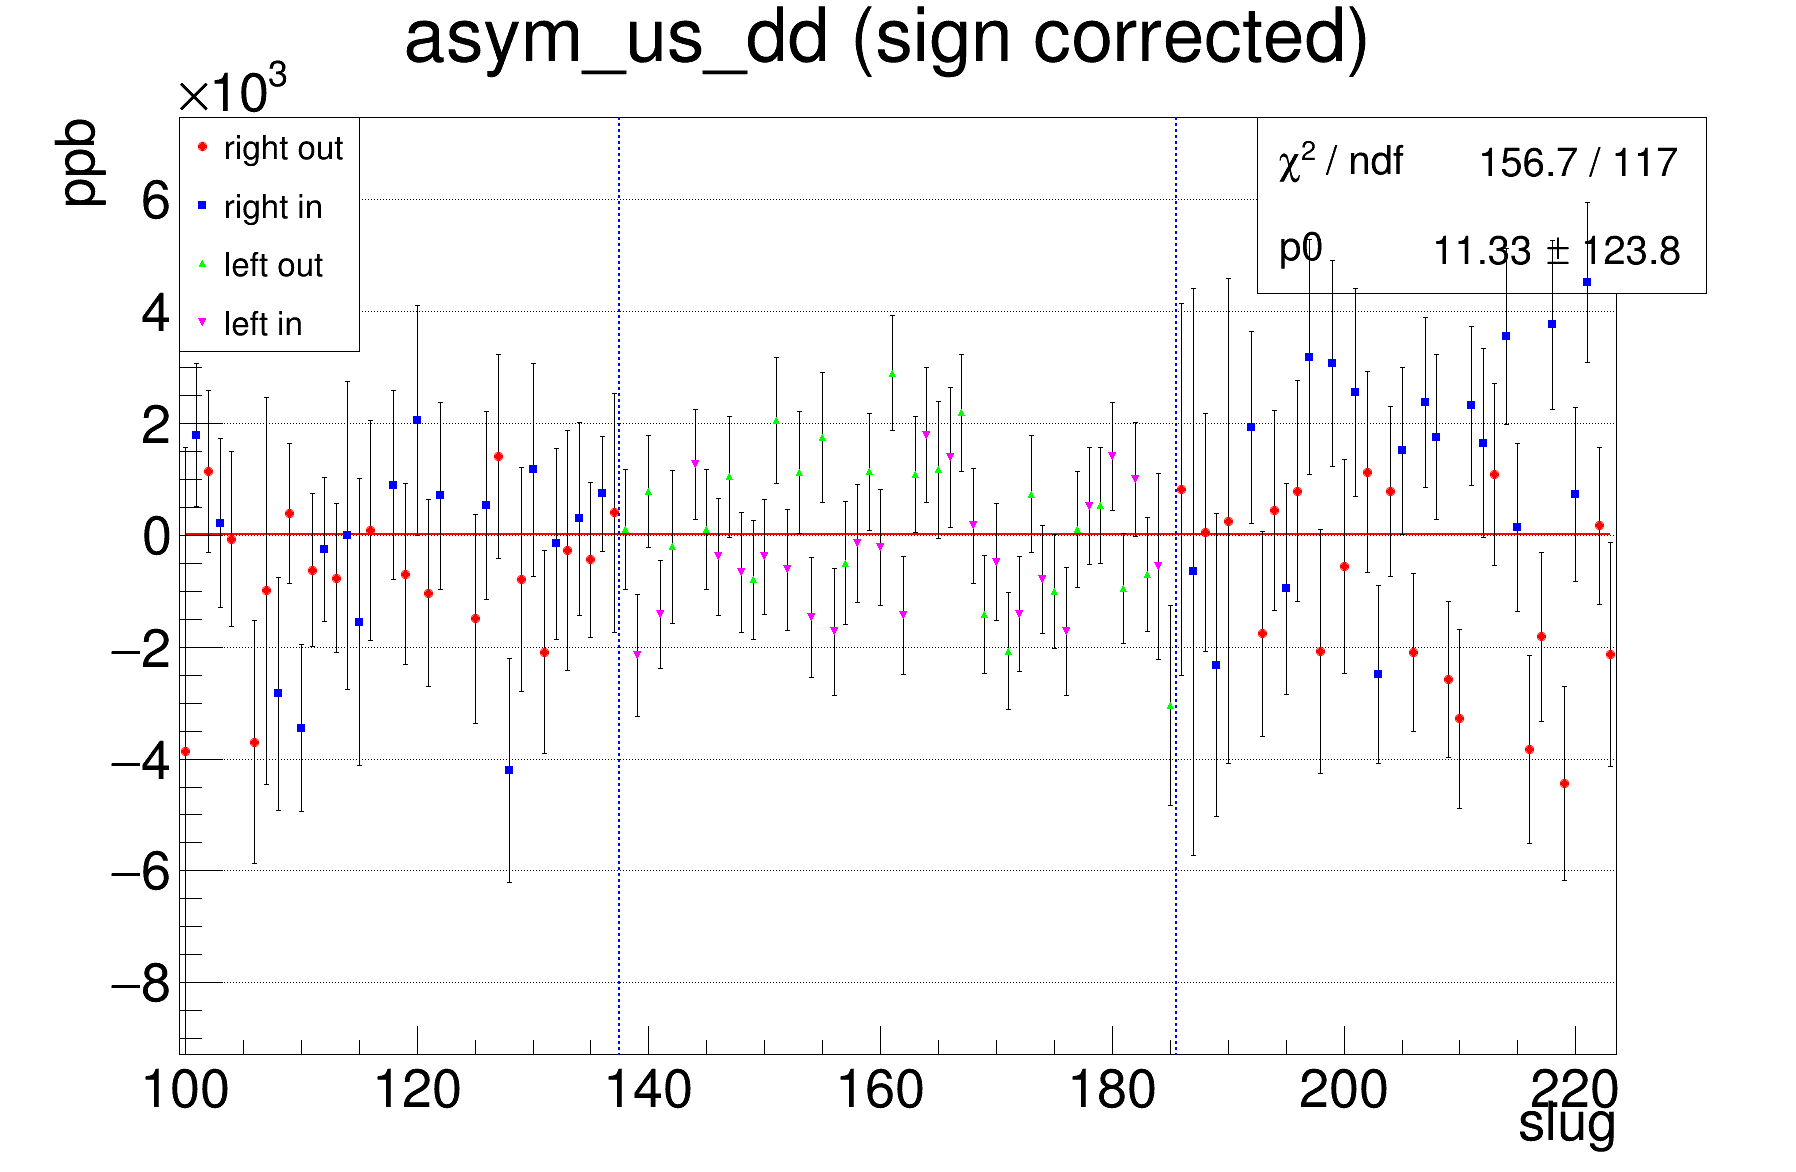
\includegraphics[width=0.49\linewidth]{crex_asym_us_dd}
    \caption{Slug-wise raw asymmetry average and difference for CREX. The right plot
    has 3 less slug because there are 3 single-arm slugs.}
\end{figure}

\begin{figure}[H]
    \centering
    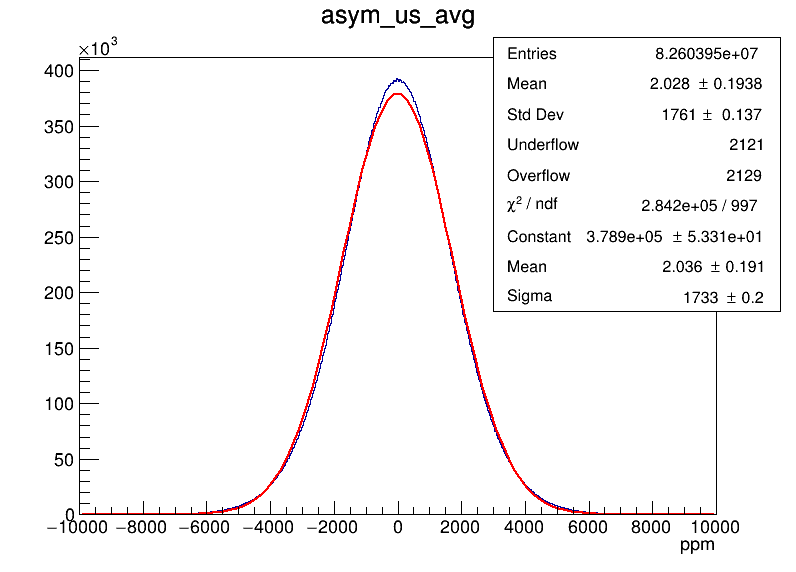
\includegraphics[width=0.49\linewidth]{crex_mulplot_asym_us_avg}
    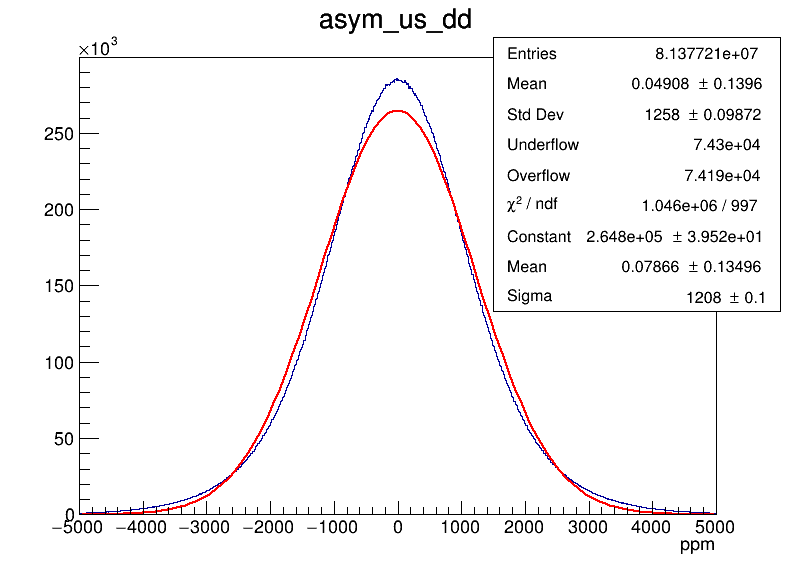
\includegraphics[width=0.49\linewidth]{crex_mulplot_asym_us_dd}
    \caption{Mulplot of CREX raw asymmetry average and difference. The blue line
    is the data and the red line is a Gaussian fit. 
    The difference plot has less entries because single arm runs have no difference.}
\end{figure}


%%%%%%%%%%%%%%%%%%%%%%%%%%%%%%%%%%%%%%%%%%%%%%%%%%%%%%%%%%%%%%%%%%%%%%%%
\section{Beam False Asymmetry Correction}
As we can see in previous few plots about beam conditions, there were false
asymmetries caused by the beam. The Helicity Correlated Beam Asymmetry (HCBA), 
was the largest contributor to false asymmetry.

As we can notice in Fig.~\ref{fig:correlation}, beam jitter will cause 
fluctuation in detector yield, with approximately a linear correlation.
So to remove the false asymmetries caused by beam jitter, we just need to
know the correlation between detector's yield and each beam parameter, what
we call the detector slope. 

\begin{figure}[H]
    \centering
    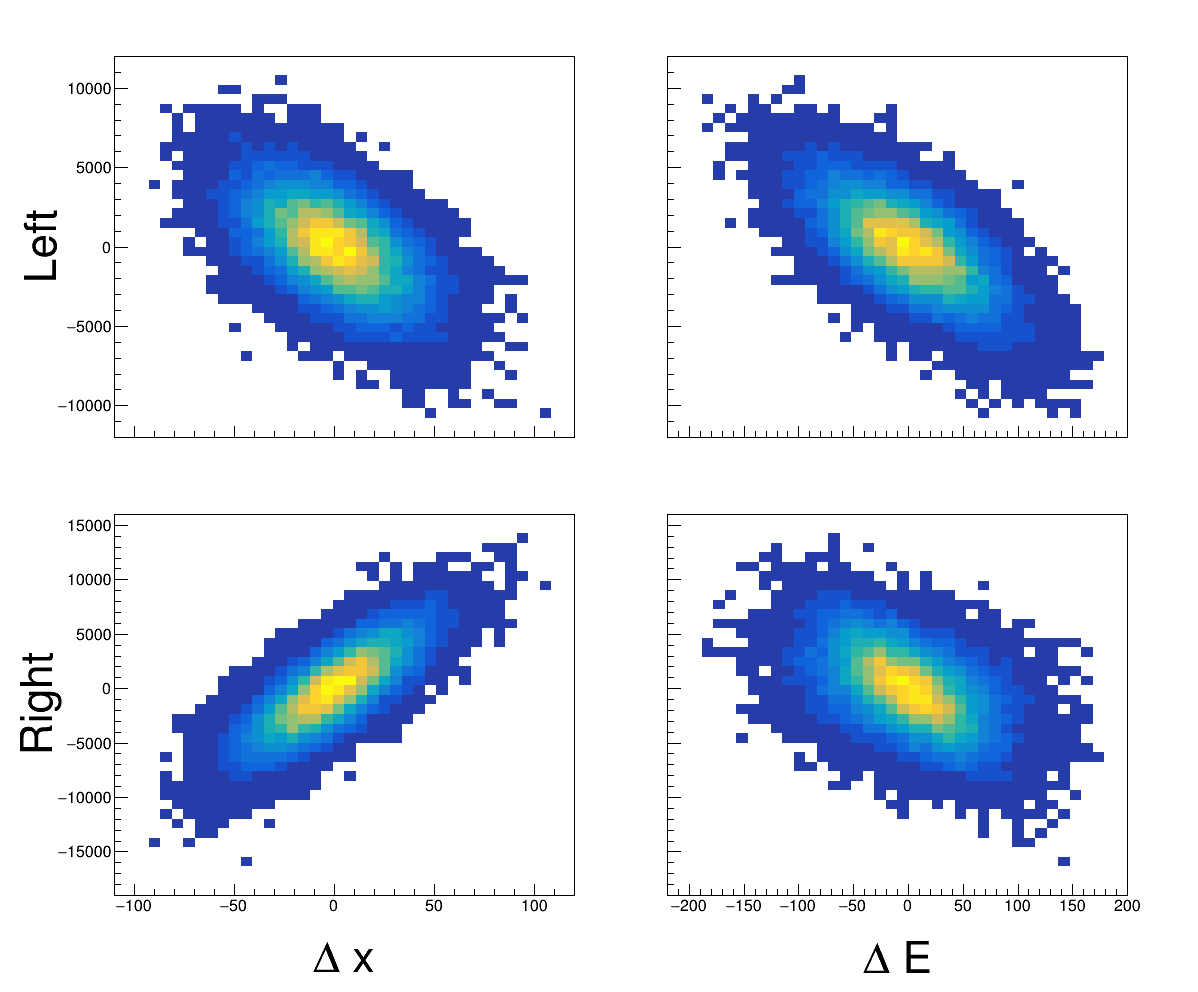
\includegraphics[width=0.6\linewidth]{run7679_correlation}
    \caption{Correlation between detector yield and beam position/energy in run 7679.}
    \label{fig:correlation}
\end{figure}

There are 2 methods to calculate the slope value, regression and beam modulation,
we will discuss them in details in the following sections.

%%%%%%%%%%%%%%%%%%%%%%%%%%%%%%%%%%%%%%%%%%%%%%%%
\subsection{Regression}

The first method to calculate the slope is regression -- a perfect scheme for
the application of the most common statistical tool, to extract the correlation
between detector yield and beam parameters.

Bear in mind that regression itself doesn't tell us any relationships or rules, 
it only works under
the assumption that the relationship of variables is predictable (given by the user) 
and the dependent variables follow a known distribution function $P(\epsilon)$, 
again, needed to be told by the user:
$$ Y = f(X) + \epsilon $$
With these prior knowledge, regression is able to calculate the most likely 
coefficients in the predicted model.

\begin{comment}
For example, the famous least square fit is actually a linear regression 
$$ Y = c_0 + \sum c_i x_i + \epsilon $$
assuming Gaussian distribution of the dependent variable: $\epsilon \sim N(0, \sigma)$
Another frequenctly used scene is logistic regression for classification, which
is very similar to linear regression except f(X) will be converted into a
probability function, e.x. using the logistic function:
$$ h(z) = \frac{e^z}{1 + e^z} \quad z = f(X) $$

The assumpsion we made here is that the fluctuations in beam parameters in small, 
compared to their normal yield -- this can be verified by their yield plot. So
that we can use first order fit to model the detector's response to change in
beam parameters. Therefore the `true' asymmetry will be:
\begin{equation}
    \CA_{cor} = \CA_{raw} - \sum_i \beta_i\Delta M_i
\end{equation}
where $\CA_{cor}$ is the corrected asymmetry, $\beta_i = \frac{\partial \CA_{raw}}{\Delta M_i}$ 
is the slope and $\Delta M$ is the difference of BPM yield bewtween 
opposite helicities windows, i sums over all 5 chosen BPMs.
\end{comment}

%%%%%%%%%%%%%%%%%%%%%%%%
\subsubsection{The Model}
Considering one monitor and one detector. Assuming the reading noise of detector
follows the Gaussian distribution and the monitor is precise (absorb the monitor
noise into beam fluctuation):
\begin{equation*}
    \begin{gathered}
	M = m	\\
	D = d + \epsilon(0, \sigma_0^D)    \\
    \end{gathered}
\end{equation*}
Here, M (D) is the measured value while m (d) is the true value and $\sigma_0^D$ 
is the variance of the noise for Detector.

Then the difference between beams of opposite polarization will follow also
the Gaussian distribution with a larger variance:
\begin{equation*}
    \begin{gathered}
	\Delta M = M^+ - M^- = m^+ - m^- = \Delta m_0   \\
	\Delta D = D^+ - D^- = (d^+ + \epsilon(0, \sigma_0^D)) - (d^- + \epsilon(0, \sigma_0^D))
	    = \Delta d_0 + \epsilon(0, \sqrt{2}\sigma_0^D)
	    = \Delta d_0 + \epsilon(0, \sigma_1^D) \\
    \end{gathered}
\end{equation*}
Again, $\Delta m_0$ ($\Delta d_0$) is the real difference between the
different polarized beams while $\Delta M$ ($\Delta D$) is the measured value.

The probability for measuring $\Delta D$ will be:
\begin{equation*}
    \begin{gathered}
	P(\Delta D) = \frac{1}{\sigma_1^D\sqrt{2\pi}} e^{-\frac{1}{2}\left( \frac{\Delta D - \Delta d_0}{\sigma_1^D}\right)^2}    \\
    \end{gathered}
\end{equation*}

We will have a bunch of independent data points: $(\Delta M, \Delta D)_i$ and 
we want to extract the relationship between $\Delta d_0$ and $\Delta m_0$: 
$\beta \equiv \frac{\partial d}{\partial m}$. Given the tininess of $\delta m$ (
compared to their normal yield), first order correlation is precise enough. 
This is exactly a linear regression problem.
\begin{equation}
    \begin{gathered}
	\Delta d = 0 + \beta \Delta m	\\
	\CA_{cor} = \CA_{raw} - \beta\Delta M	\\
    \end{gathered}
\end{equation}

For any real data point $(\Delta m_0, \Delta d_0)_i$, the possibility to measure
$(\Delta M, \Delta D)_i$ is:
\begin{equation}
    \begin{gathered}
	P_i(\Delta D|\Delta M) = \frac{1}{\sigma_1^D\sqrt{2\pi}} 
	    e^{-\frac{1}{2}\left( \frac{\Delta D - \beta\Delta M}{\sigma_1^D}\right)^2}
    \end{gathered}
\end{equation}

For the accumulated data of one minirun, the total probability will be:
\begin{equation}
    P = \prod_i^n P_i(\Delta D|\Delta M) = \prod_i^n \frac{1}{\sigma_1^D\sqrt{2\pi}} 
	    e^{-\frac{1}{2}\left( \frac{\Delta D_i - \beta\Delta M_i}{\sigma_1^D}\right)^2}
\end{equation}

To maximize P, it is equivalently to minimize:
\begin{equation}
    \chi^2 = \sum_i (\Delta D - \beta\Delta M)_i^2
    \label{eqn:regression_chi2}
\end{equation}
where i sums over all samples in one minirun.

We will have:
\begin{equation}
    \frac{\partial P}{\partial \beta} = P \times 
    \sum_i \frac{\Delta M_i}{\sigma_1^D} \left( \frac{\Delta D_i - \beta\Delta M_i}{\sigma_1^D}\right)
    = 0
\end{equation}
Which gives $\beta$ as:
\begin{equation}
    \sum_i \Delta M_i (\Delta D_i - \beta\Delta M_i) = 0  \quad \Rightarrow \quad
    \beta = \frac{\sum \Delta D_i \Delta M_i}{\sum \Delta M^2_i}
\end{equation}

Extend independent variable to multi-dimensional, we have:
\begin{equation}
    \Delta D = \begin{pmatrix} \beta_1 & \beta_2 & \cdots & \beta_m \end{pmatrix} 
	\begin{pmatrix}
	    \Delta M^1	\\
	    \Delta M^2	\\
	    \vdots 	\\
	    \Delta M^m	\\
	\end{pmatrix}
	+ \epsilon(0, \sigma^D)
\end{equation}
where m is the number of used BPMs.
\begin{equation}
    \frac{\partial P}{\partial \beta_\nu} \propto \sum_i \Delta M_i^\nu (\Delta D_i - \sum_\mu \beta_\mu M_i^\mu) = 0
\end{equation}
Arrange them in a matrix:
\begin{equation}
    \small
    \begin{pmatrix}
	\sum_i \Delta D_i \Delta M_i^1 \\
	\sum_i \Delta D_i \Delta M_i^2 \\
	\vdots	\\
	\sum_i \Delta D_i \Delta M_i^m \\
    \end{pmatrix}
    = 
    \begin{pmatrix}
	\sum_i \Delta M_i^1 \Delta M_i^1    & \sum_i \Delta M_i^1 \Delta M_i^2	&
	\cdots	& \sum_i \Delta M_i^1 \Delta M_i^m  \\
	\sum_i \Delta M_i^2 \Delta M_i^1    & \sum_i \Delta M_i^2 \Delta M_i^2	&
	\cdots	& \sum_i \Delta M_i^2 \Delta M_i^m  \\
	\vdots	& \vdots    & \ddots	& \vdots    \\
	\sum_i \Delta M_i^m \Delta M_i^1    & \sum_i \Delta M_i^m \Delta M_i^2	&
	\cdots	& \sum_i \Delta M_i^m \Delta M_i^m  \\
    \end{pmatrix}
    \begin{pmatrix}
	\beta_1 \\
	\beta_2 \\
	\vdots	\\
	\beta_m \\ 
    \end{pmatrix}
\end{equation}

Define covariance of any 2 variables as:
\begin{equation}
    cov(x, y) = \sum_i x_i y_i
\end{equation}
and
\begin{equation}
    M_{m \times m} = 
    \begin{pmatrix}
	cov(\Delta M^1, \Delta M^1) & cov(\Delta M^1, \Delta M^2)   & \cdots & cov(\Delta M^1, \Delta M^m)  \\
	cov(\Delta M^2, \Delta M^1) & cov(\Delta M^2, \Delta M^2)   & \cdots & cov(\Delta M^2, \Delta M^2)  \\
	\vdots	& \vdots    & \ddots	& \vdots    \\
	cov(\Delta M^m, \Delta M^1) & cov(\Delta M^m, \Delta M^2)   & \cdots & cov(\Delta M^m, \Delta M^m)  \\
    \end{pmatrix}
\end{equation}

To get:
\begin{equation}
    \begin{pmatrix}
	\beta_1 \\
	\beta_2 \\
	\vdots	\\
	\beta_m \\ 
    \end{pmatrix}
    =
    M^{-1}
    \begin{pmatrix}
	cov(\Delta D, \Delta M^1)   \\
	cov(\Delta D, \Delta M^2)   \\
	\vdots	\\
	cov(\Delta D, \Delta M^m)   \\
    \end{pmatrix}
\end{equation}

\begin{comment}
For multiple detectors, it is easy to get:
\begin{equation}
    \small
    \begin{aligned}
	\begin{pmatrix}
	    \beta_{11}	& \beta_{21}    & \cdots & \beta_{m1}	\\
	    \beta_{12}	& \beta_{22}    & \cdots & \beta_{m2}	\\
	    \vdots	& \vdots    & \ddots	& \vdots\\
	    \beta_{1n}	& \beta_{2n}    & \cdots & \beta_{mn}	\\
	\end{pmatrix}
	&= A^{-1}
	&\times
	\begin{pmatrix}
	    cov(\Delta D^1, \Delta M^1) & cov(\Delta D^2, \Delta M^1)   & \cdots	& cov(\Delta D^m, \Delta M^1)	\\
	    cov(\Delta D^1, \Delta M^2) & cov(\Delta D^2, \Delta M^2)   & \cdots	& cov(\Delta D^m, \Delta M^2)	\\
	    \vdots	& \vdots    & \ddots	& \vdots    \\
	    cov(\Delta D^1, \Delta M^n) & cov(\Delta D^2, \Delta M^n)   & \cdots	& cov(\Delta D^m, \Delta M^n)	\\
	\end{pmatrix}
    \end{aligned}
    \label{eqn:slope}
\end{equation}
where $\beta_{ij}$ refers to detector i's response to change in monitor j.
\end{comment}

Theoretically and practically, we need only 5 BPMs to cover all the beam motion phase space.
The 5 BPMs we chose in CREX analysis were BPM1X, BPM4aY, BPM4eX, BPM4eY and BPM12X.

%%%%%%%%%%%%%%%%%%%%%%%%
\subsubsection{Slope Values}
With Eq.~\ref{eqn:slope}, we can calculate the slope values w.r.t. to chosen 
BPMs. Fig.~\ref{fig:slug_202_reg_asym_us_avg_diff_bpm12X} justifies our usage
of minirun. As we can see in the plot, the slope value depends on the detector 
yield, miniruns within the same run may have different slope values up to a few 
percent. This is expected because we assumed the Gaussian distribution
of the detector yield. So small shift in beam conditions change the detector
yield, and therefore the slope values. A minirun-wise slope value is more stable
than a run-wise one, and correct the false asymmetry more precisely. This also
means that the regression correction can deal with only small fluctuation around 
mean value, it is imprecise to do the same correction for outliers, that's why
we need to remove miniruns with beam condition outliers.
\begin{figure}[H]
    \centering
    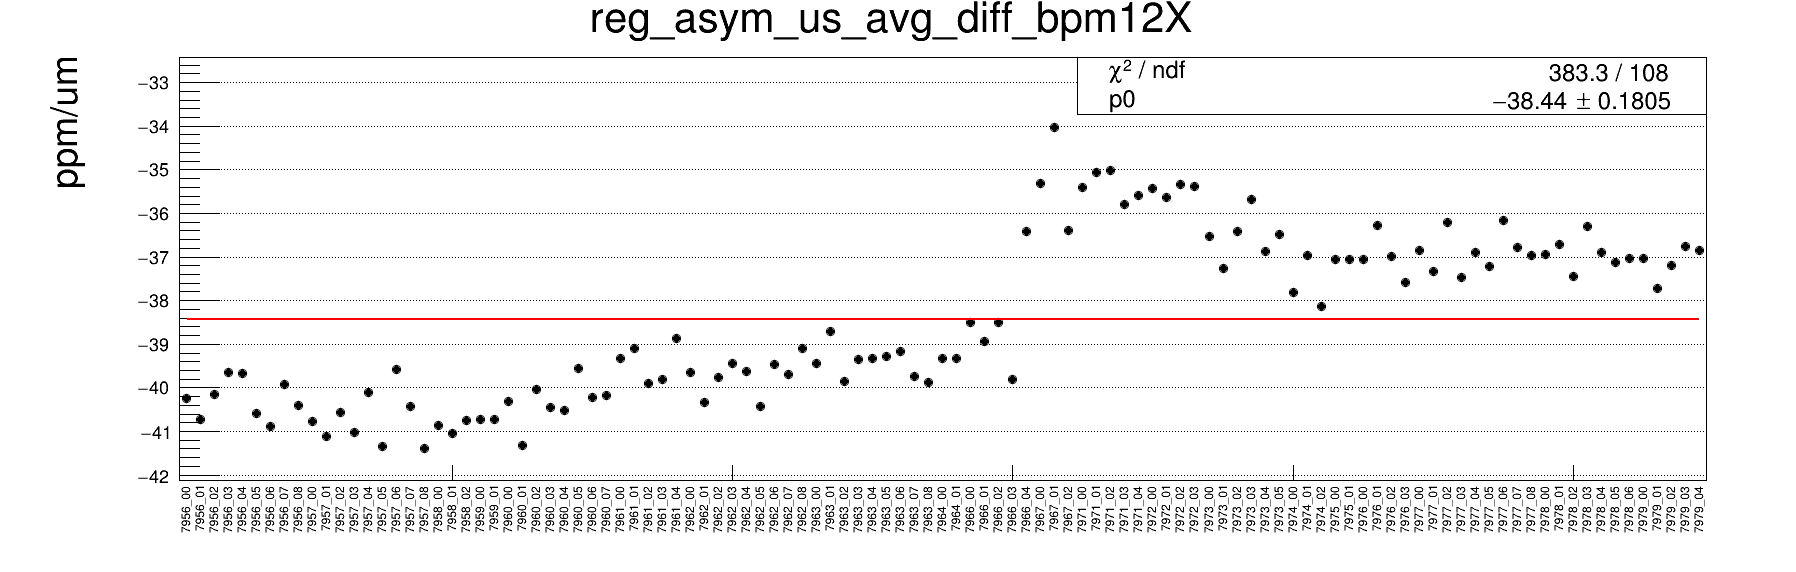
\includegraphics[width=\linewidth]{slug_202_reg_asym_us_avg_diff_bpm12X}
    \caption{Slope value w.r.t. to BPM12X of each minirun in slug 202, the X-axis 
    is the run number attached by minirun number.}
    \label{fig:slug_202_reg_asym_us_avg_diff_bpm12X}
\end{figure}

Table~\ref{tab:crex_slope} summarise the approximating slope values w.r.t. the 5
BPMs we chose. Overall, our detector is sensitive to fluctuations in X direction
(the disperse direction) and beam energy, and dull to jitters in Y direction.
\begin{table}[!h]
    \centering
    \begin{tabular}{c | c}
	\hline
	BPM & slope ($ppm/\mu m$)   \\
	\hline
	1X  & $\sim -40$    \\
	4aY & $\sim 15$    \\
	4eX & $\sim 40$	\\
	4eY & $\sim 0$	\\
	12X & $\sim -40$    \\
	\hline
    \end{tabular}
    \caption{Slope values w.r.t. different BPMs.}
    \label{tab:crex_slope}
\end{table}

%%%%%%%%%%%%%%%%%%%%%%%%
\subsubsection{Corrections}
With the slope value for each monitor, we can calculate the corresponding
false asymmetry correction:
\begin{equation}
    \CA_{cor} = \beta \times \text{(diff in bpm)}
\end{equation}
The main correction comes from difference in X direction and energy,
typical correction is about a few ppm, as shown in Fig.~\ref{fig:slug_202_reg_asym_us_avg_diff_bpm12X}.
Due to detector's insensitivity to fluctuation in the Y direction, its correction 
is relatively small, at the level of  a few hundred $ppb$. Note that corrections
from each beam parameter don't add up, they actually cancel with each other,
leaving relatively small total correction, usually a few $ppm$.

\begin{figure}[H]
    \centering
    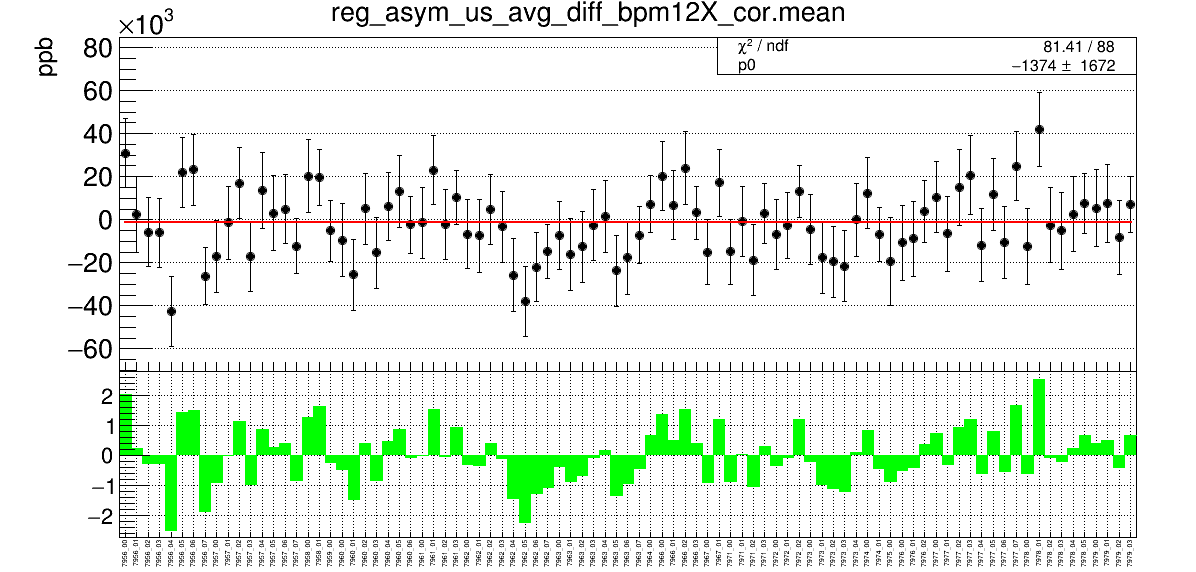
\includegraphics[width=\linewidth]{slug_202_reg_asym_us_avg_diff_bpm12X_cor.mean}
    \caption{False asymmetry corection caused by energy difference (bpm12X) in
    slug 202.}
    \label{fig:slug_202_reg_asym_us_avg_diff_bpm12X_cor}
\end{figure}

\begin{table}[!h]
    \centering
    \begin{tabular}{c | c}
	\hline
	BPM  & correction   \\
	\hline
	1X  & a few tenths $ppm$ \\
	4aY & a few hundreds $ppb$     \\
	4eX & a few tentehs $ppm$ \\
	4eY & a few hundreds $ppb$     \\
	12X  & a few tenths $ppm$ \\
	\hline
    \end{tabular}
    \caption{Typical false asymmetry corection from each bpm.}
\end{table}

%%%%%%%%%%%%%%%%%%%%%%%%
\subsubsection{Regression Result}
The asymmetry after regression correction reads $2080 \pm 84.01\ ppb$, as shown 
in the left plot of Fig.~\ref{fig:reg_asym_us_avg}. Compared to the raw asymmetry
of $2106 \pm 178.9\ ppb$,
the mean value doesn't change much, which is expected because the assumption 
we made is that the false asymmetry follows the Gaussian distribution, therefore
regression should just remove the noise without changing the mean value, which
is exactly what we got. The width of the asymmetry distribution after regression
reduces by a factor of 2, as shown in the right plot of Fig.~\ref{fig:reg_asym_us_avg}.

\begin{figure}[H]
    \centering
    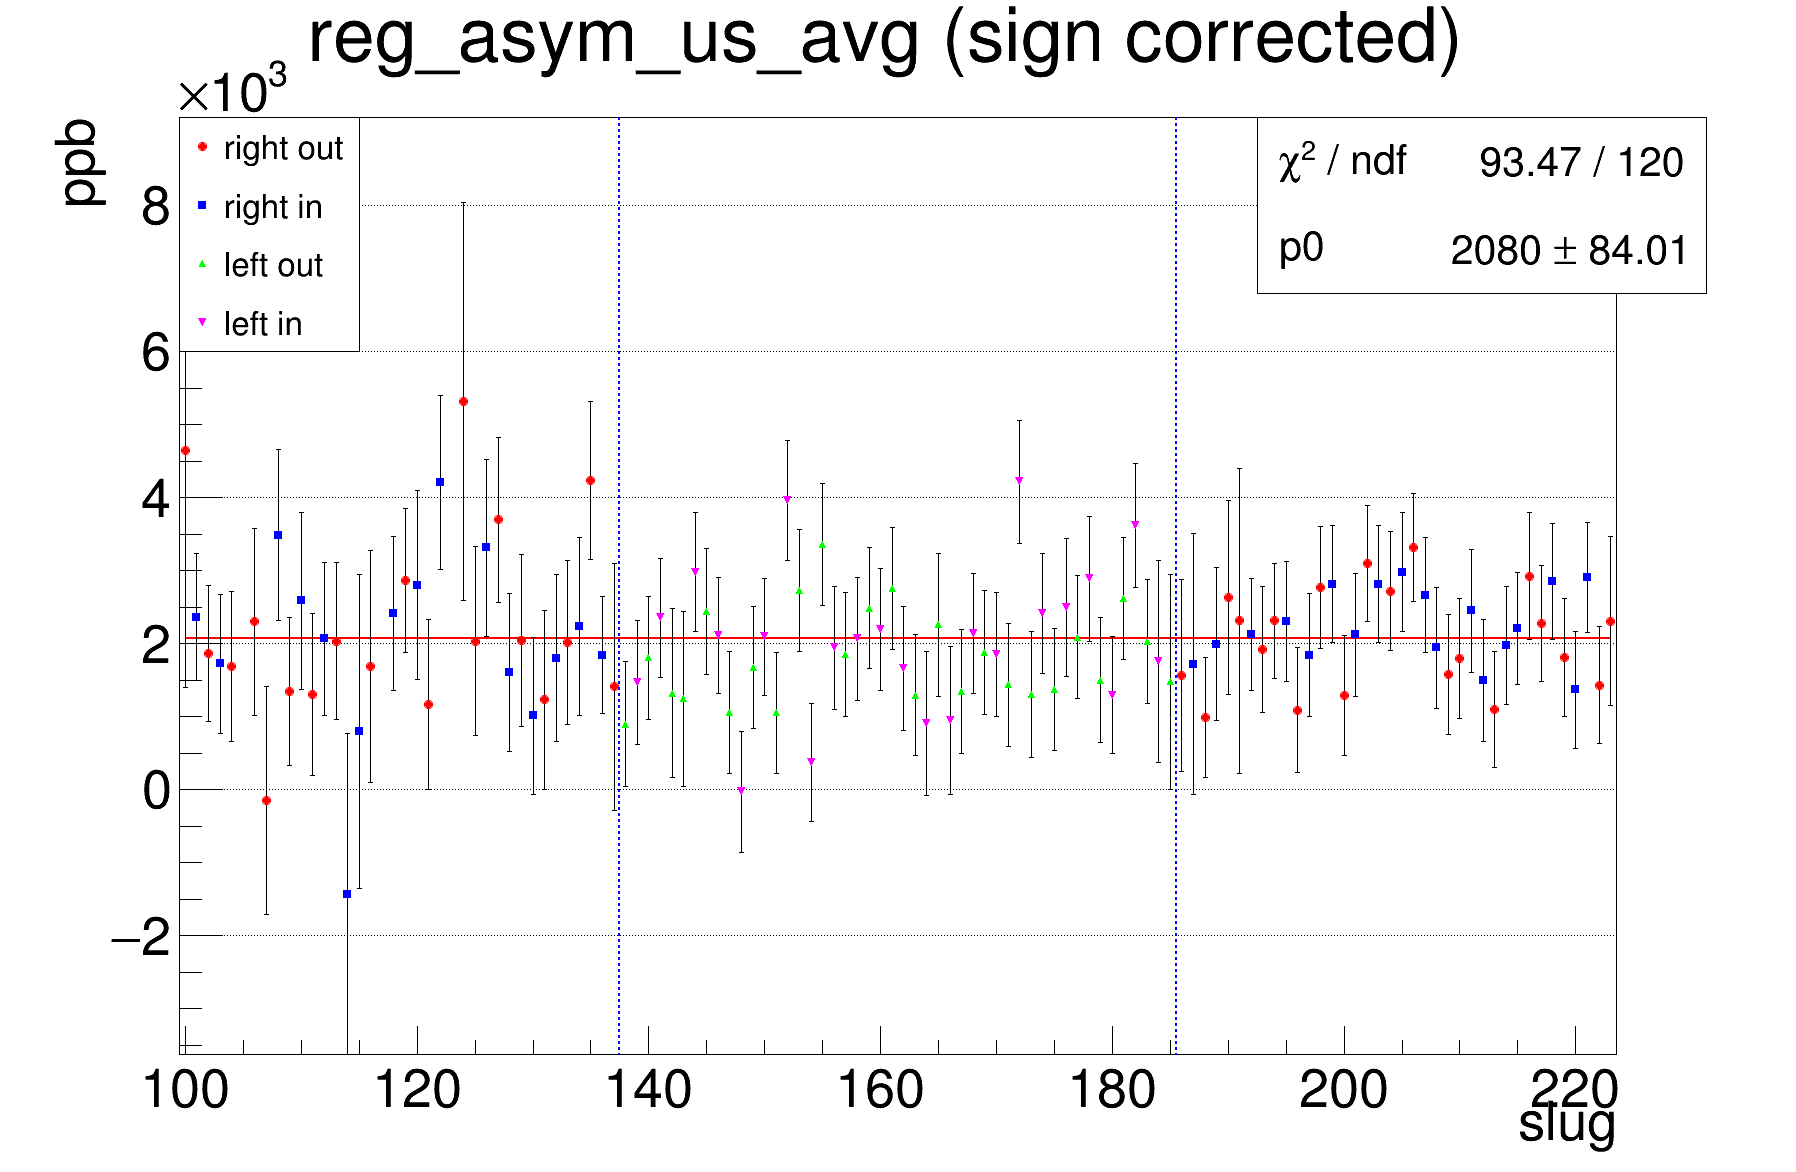
\includegraphics[width=0.52\linewidth]{crex_reg_asym_us_avg}
    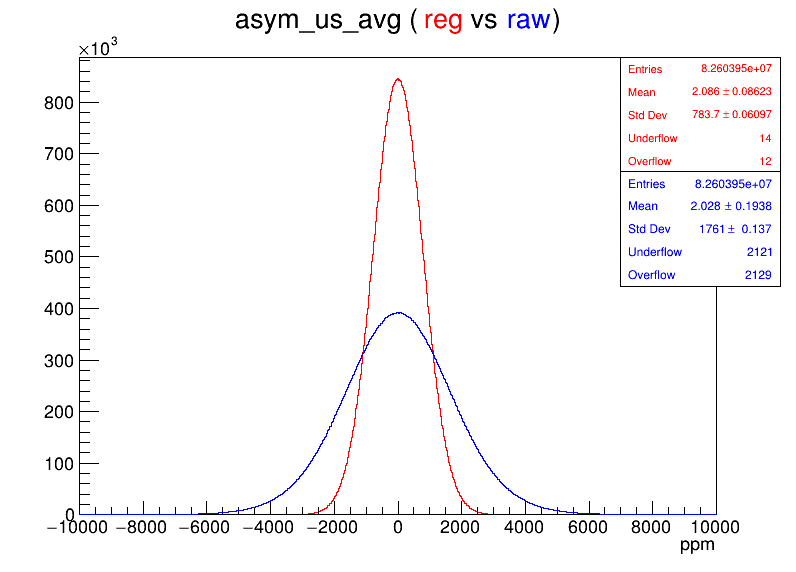
\includegraphics[width=0.47\linewidth]{crex_mulplot_asym_us_avg_cor}
    \caption{Left: asymmetry of each slug after regression correction.
    Right: Comparison of asymmetry distributions before and after regression correction.}
    \label{fig:reg_asym_us_avg}
\end{figure}

%%%%%%%%%%%%%%%%%%%%%%%%
\subsubsection{Null Result}
One way to check the correctness of our result is the null asymmetry, which
is the difference between the LHRS and RHRS asymmetry (divided by 2). 
In ideal case, the null asymmetry should be 0. Our measurement shows exactly
the expectation, the corrected null asymmetry is about $85\ ppb$, very close
to 0.
\begin{figure}[H]
    \centering
    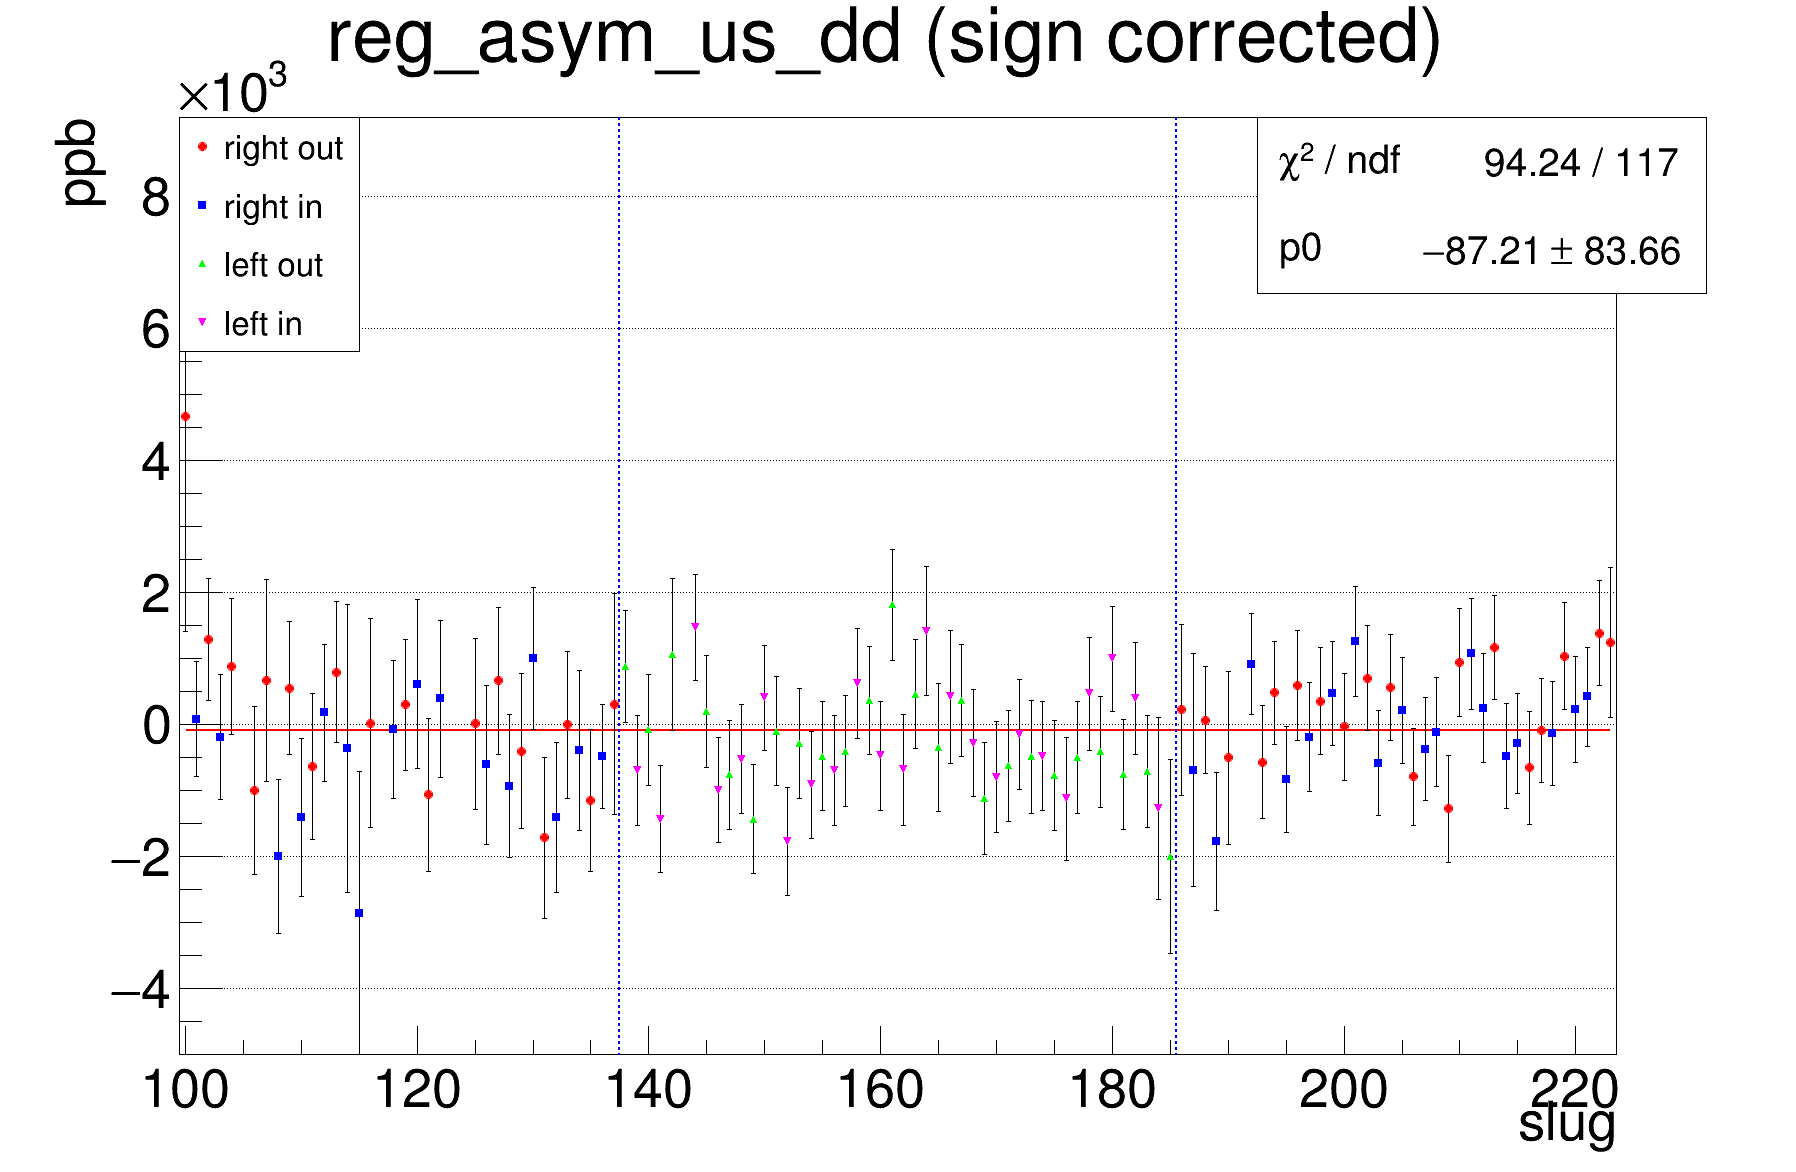
\includegraphics[width=0.52\linewidth]{crex_reg_asym_us_dd}
    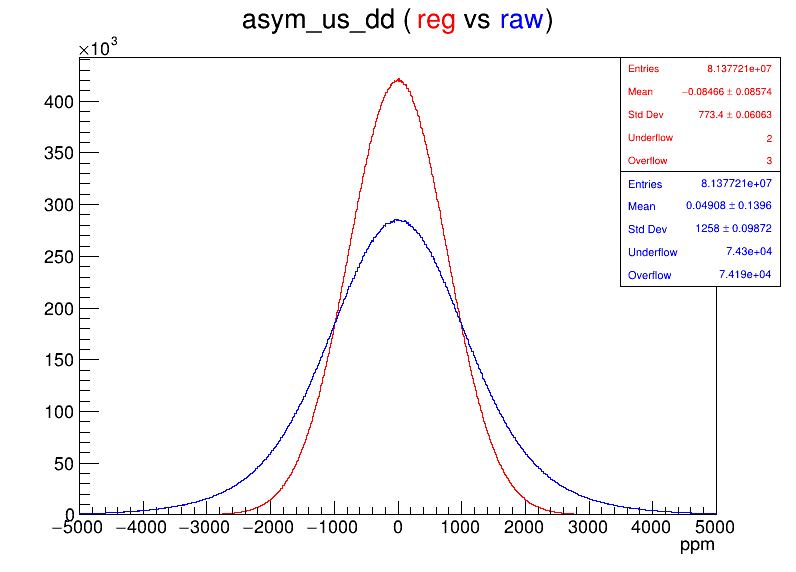
\includegraphics[width=0.47\linewidth]{crex_mulplot_asym_us_dd_cor}
    \caption{Asymmetry after regression correction.}
    \label{fig:reg_asym_us_dd}
\end{figure}

%%%%%%%%%%%%%%%%%%%%%%%%%%%%%%%%%%%%%%%%%%%%%%%%
\subsection{Beam Modulation}
Another way to do the beam false asymmetry correction is beam modulation. After
all, if we want to know detector's response to beam fluctuations, we can measured
it directly -- which is beam modulation. By modulating beam position/angle/energy
intentionally, changes measured in monitors and detectors will tell us the slope.
The key point is to make sure the modulating amplitude is larger than that of 
natural beam fluctuation, so that we can extract the real response.

\begin{figure}
    \centering
    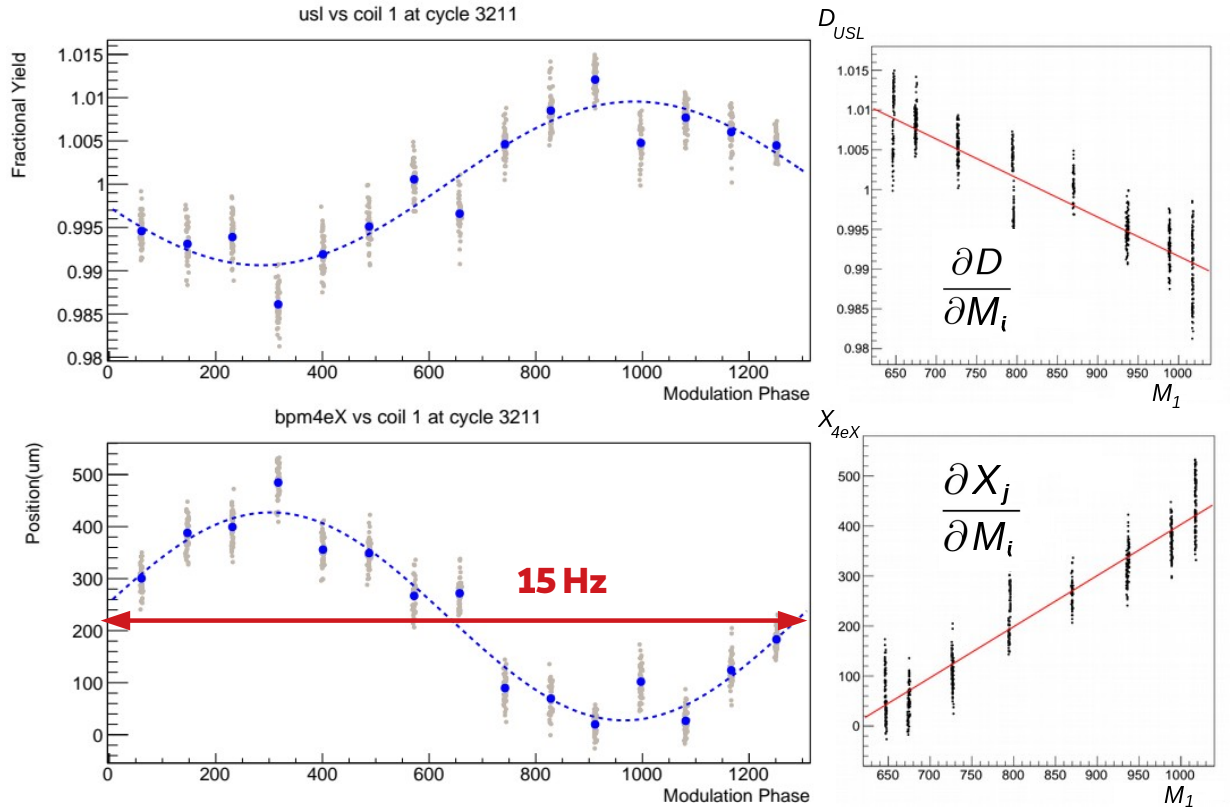
\includegraphics[width=0.7\linewidth]{modulation_cycle3211}
    \caption{An example of beam modulation.}
\end{figure}

To express the idea mathematically, let D (M) be the Detector (Monitor) yield and C be
the modulation coil input, we have:
\begin{equation}
    \frac{\partial D}{\partial C_\alpha} = \sum_\mu \frac{\partial D}{\partial M_\mu}\frac{\partial M_\mu}{\partial C_\alpha}
\end{equation}
or in an alternative form:
\begin{equation}
    \frac{\partial D}{\partial M_\mu} = \sum_\alpha \frac{\partial D}{\partial C_\alpha}\frac{\partial C_\alpha}{\partial M_\mu} = \sum_\alpha \frac{\partial D}{\partial C_\alpha}\left(\frac{\partial M_\mu}{\partial C_\alpha}\right)^{-1}
\end{equation}
the slope value $\frac{\partial D}{\partial M}$ is what we want to know.

Define matrix B as:
\begin{equation}
    B_{n \times m} = 
    \begin{pmatrix}
	\frac{\partial M_1}{\partial C_1}   & \frac{\partial M_2}{\partial C_1}	& \cdots  & \frac{\partial M_m}{\partial C_1}   \\
	\frac{\partial M_1}{\partial C_2}   & \frac{\partial M_2}{\partial C_2}	& \cdots  & \frac{\partial M_m}{\partial C_2}   \\
	\vdots	& \vdots    & \ddots	& \vdots    \\
	\frac{\partial M_1}{\partial C_n}   & \frac{\partial M_2}{\partial C_n}	& \cdots  & \frac{\partial M_m}{\partial C_n}   \\
    \end{pmatrix}
\end{equation}
to get:
\begin{equation}
    \begin{pmatrix}
	\frac{\partial D}{\partial M_1}	\\
	\frac{\partial D}{\partial M_2}	\\
	\vdots	\\
	\frac{\partial D}{\partial M_n}	\\
    \end{pmatrix}
    =
    B^{-1}
    \begin{pmatrix}
	\frac{\partial D}{\partial C_1}	\\
	\frac{\partial D}{\partial C_2}	\\
	\vdots	\\
	\frac{\partial D}{\partial C_n}	\\
    \end{pmatrix}
\end{equation}

To make the matrix B invertable, we must have
\begin{equation}
    n = m
\end{equation}
which is the same number of monitors and coils.

The calculation of sensitivity is the same as we calculate the regression slope:
\begin{equation}
    \frac{\partial D}{\partial C} = \frac{cov(D, C)}{\bar{D} \cdot cov(C, C)}
    \qquad
    \frac{\partial M}{\partial C} = \frac{cov(M, C)}{\bar{M} \cdot cov(C, C)}
\end{equation}
where $\bar{D}$ is the averge detector yield and $cov$ is the covariance. The
mean yield in the denominator is for normalization. 

These sensitivities and their combinations were used for beam monitoring during
data taking, to alarm possible large beam fluctuations.

%%%%%%%%%%%%%%%%%%%%%%%%
\subsubsection{Run Segments}
As we mentioned before, the modulation system consists of 7 coils, a complete 
cycle of modulation takes about $2 mins$. Stable beam was required for modulation.
Unfortunately, with low frequency of beam modulation (about 1 modulation per 10~mins), 
it was an wild wish to have stable beam conditions during beam modulation. Chances were
beam trip off during beam modulation, resulting in incomplete cycles. Though we
need only 5 out of the total 7 coils to cover the whole beam parameter phase space,
it still hurt if we discard those cycles that don't have the chosen 5 coils. So
the strategy we chose was to calculate dithering sensitivities and slopes run-wise
using all cycles in one run, rather than cycle-wise, to make use of 
as much modulation data as possible.

Even though the run-wise strategy to save incomplete cycles, some runs were still
lack of dithering data. To enable dithering correction for these runs, we separated
runs into segments based on beam conditions. An average dithering slope value
was calculated using run-wise values within each segment and then the calculated
slope value was used for correction for each run in that segment. The separation
of segments happen when there were changes in beam setup or when we observed shift
in slope values. List of segments can be found in Cameron's thesis \cite{Cameron_thesis}.

%%%%%%%%%%%%%%%%%%%%%%%%
\subsubsection{Beam Modulation Result}
The dithering corrected asymmetry of $2085 \pm 84.22\ ppb$ is $0.24\%$ away from
regression corrected result of $2080 \pm 84.01\ ppb$, verifying the correctness
of both methods. The difference between asymmetries corrected with these 2 methods
for each slug is shown in the right plot of Fig.~\ref{fig:dit_result}, the difference
is zero within uncertainty for most slugs.
\begin{figure}[H]
    \centering
    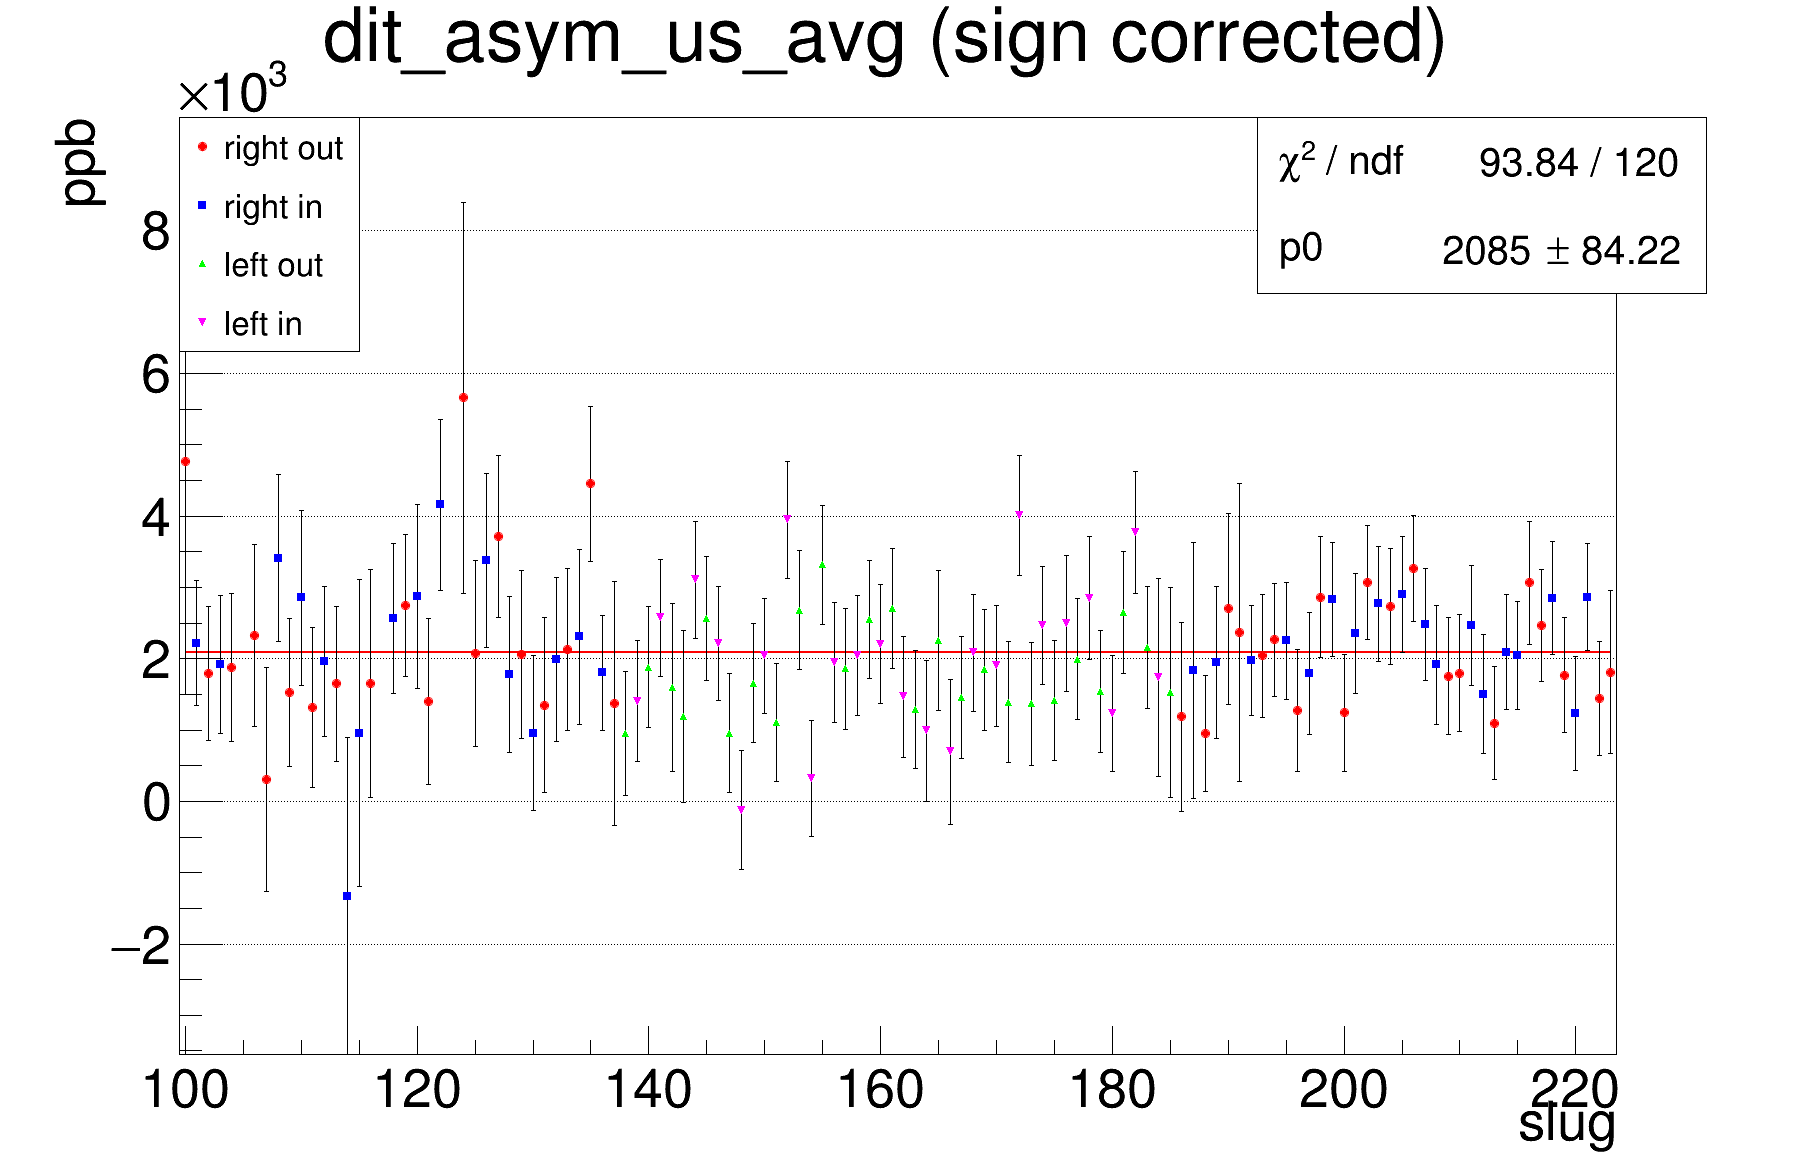
\includegraphics[width=0.49\linewidth]{crex_dit_asym_us_avg}
    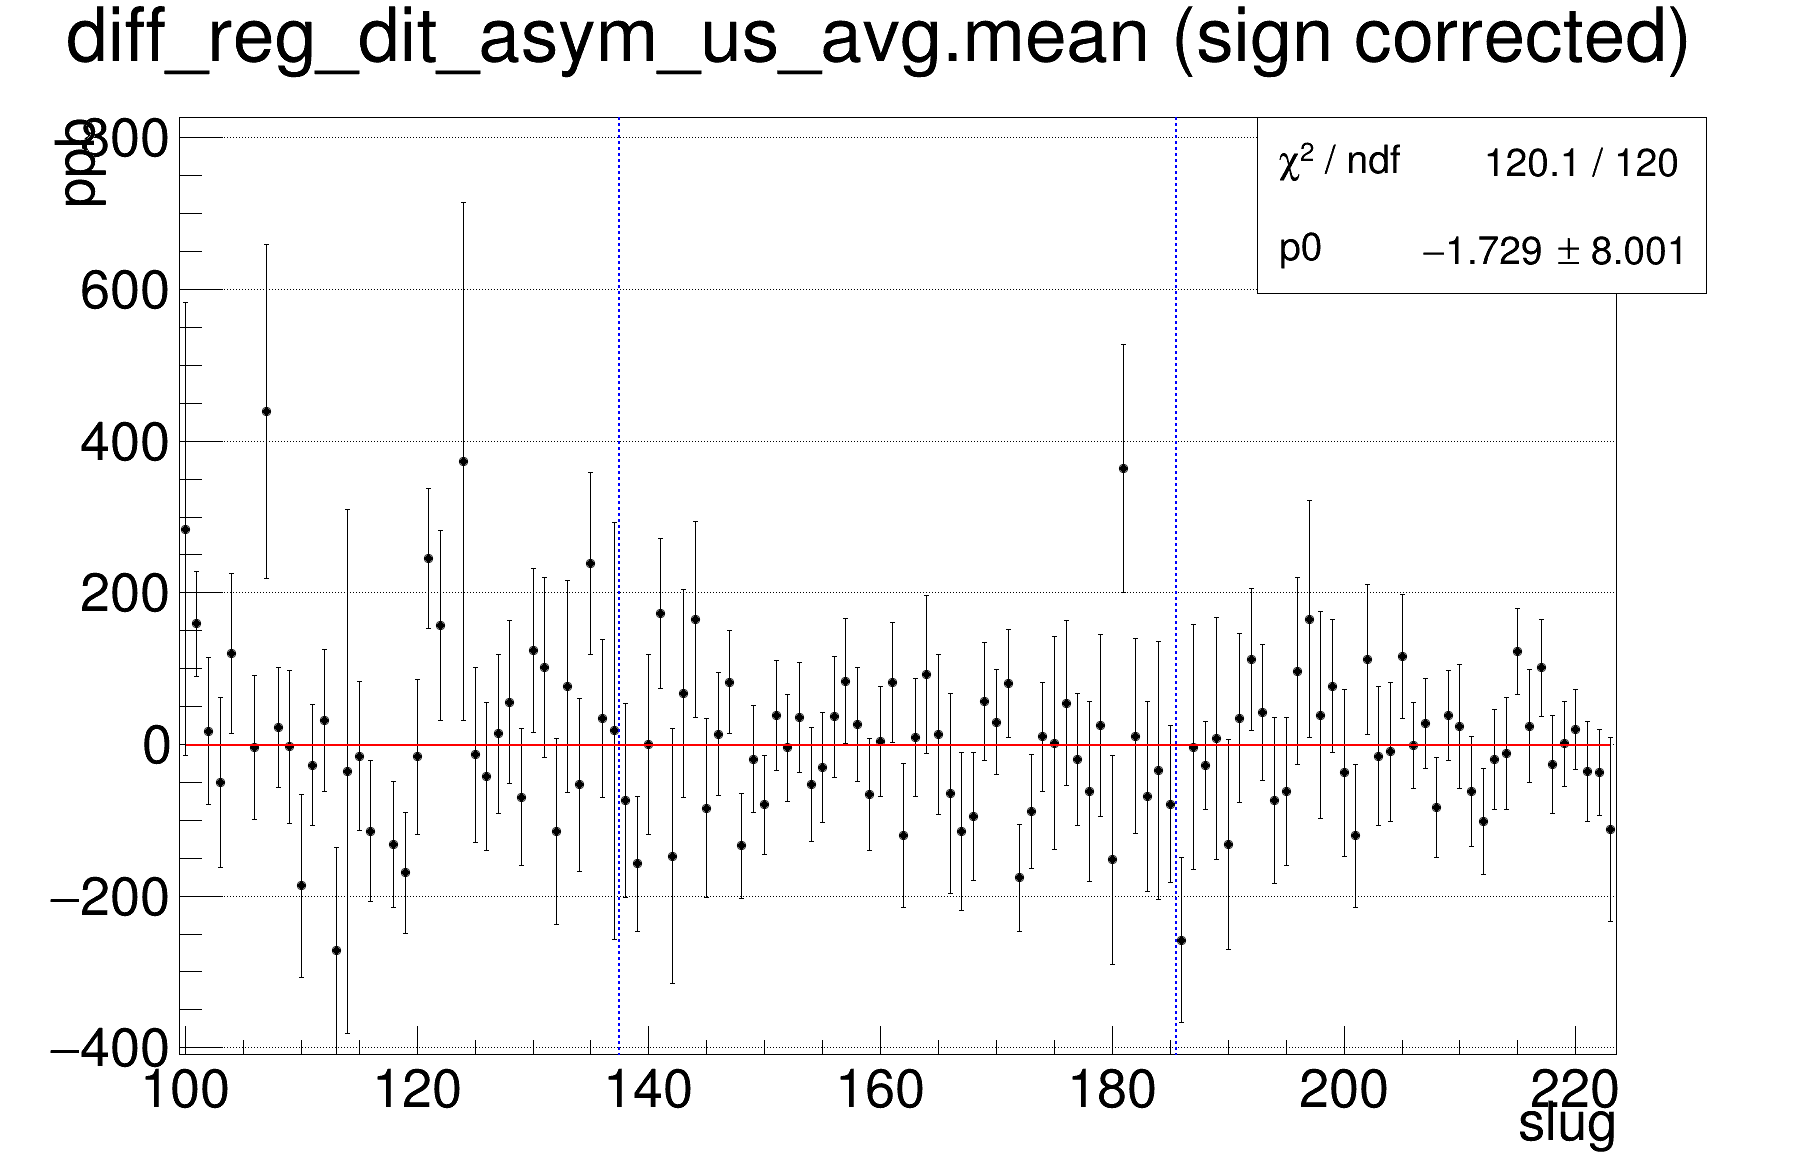
\includegraphics[width=0.49\linewidth]{crex_diff_reg_dit_asym_us_avg.mean}
    \caption{Left: Asymmetry after beam modulation correction.
    Right: difference between asymmetry values corrected by regression and
    beam modulation in each slug.}
    \label{fig:dit_result}
\end{figure}


%%%%%%%%%%%%%%%%%%%%%%%%%%%%%%%%%%%%%%%%%%%%%%%%
\subsection{Lagrange Multiplier}
As we said before, we used miniruns for more precise false asymmetry correction, 
but in dithering correction, we used segment-wise slopes due to lack of modulation
data. Though more precise than dithering correction, the regression method is 
less accurate than dithering, because of natural noise in detectors/monitors. 
The modulation amplitude is larger than the internal noise (of course, the amplitude
should keep small compare to the yield: $\lesssim 1\%$), therefore being
more accurate by suppressing the effect of those noise.

Given the advantages and disadvantages of these 2 methods, it is natural to 
combine these 2 methods, which leads to the Lagrangian analysis -- regression
with constraint from beam modulation.

From Eq.~\ref{eqn:regression_chi2}, we can derive the $chi^2$ for asymmetry regression:
\begin{equation}
    \chi^2 = \sum_i \left( \CA_{raw} - \sum_\mu \beta_\mu \Delta M_\mu \right)_i^2
\end{equation}
where n sums over samples and i sums over BPMs.

The Lagrangian multiplier for this constraint problem will:
\begin{equation}
    \CL = \sum_i \left( \CA_{raw} - \sum_\mu \beta_\mu \Delta M_\mu \right)_i^2+ \sum_\alpha \lambda_\alpha \left(\sum_\mu \beta_\mu \frac{\partial M_\mu}{\partial C_\alpha} - \frac{\partial D}{\partial C_\alpha} \right)
\end{equation}
where $\mu$ sums over selected monitors and $\alpha$ sums over selected coils.

\begin{equation}
    \begin{aligned}
	\frac{\partial \CL}{\partial \beta_\mu} &= -2\Delta M_\mu \sum_i \left( \CA_{raw} - \sum_\nu \beta_\nu \Delta M_\nu \right)_i + \sum_\alpha \lambda_\alpha \frac{\partial M_\mu}{\partial C_\alpha}    \\
	    &= 2 \left(\sum_\nu \beta_\nu \cdot cov(\Delta M_\mu, \Delta M_\nu) - cov(\CA_{raw}, \Delta M_\mu) \right) + \sum_\alpha \lambda_\alpha \frac{\partial M_\mu}{\partial C_\alpha} = 0  \\
	\frac{\partial \CL}{\partial \lambda_\alpha} &= \left( \sum_\mu \beta_\mu \frac{\partial M_\mu}{\partial C_\alpha} - \frac{\partial D}{\partial C_\alpha} \right) = 0\\
    \end{aligned}
    \label{eqn:lagrange_derivative}
\end{equation}

The difference between the second formula of Eq.~\ref{eqn:lagrange_derivative} and
the normal beam modulation method may be confusing, because they are actually
the same if we consider only 5 BPMs. The constraint from beam modulation is so 
strong that it identifies the slope values directly. Changes happen when we
include more BPMs in the analysis, with more BPMs than coils, the solution
to the constraint is not unique anymore, so that we can apply the Lagrange multiplier
method.

Write Eq.~\ref{eqn:lagrange_derivative} in matrix form:
\begin{equation}
    \begin{pmatrix}
	M_{m\times m}	& (B^T)_{m\times n}	\\
	B_{n \times m}  & \bm{0}_{n\times n}   \\
    \end{pmatrix}
    \begin{pmatrix}
	\beta_1	\\
	\vdots	\\
	\beta_m	\\
	\frac{\lambda_1}{2} \\
	\vdots	\\
	\frac{\lambda_n}{2} \\
    \end{pmatrix}
    =
    \begin{pmatrix}
	cov(\CA_{raw}, \Delta M_1)  \\
	\vdots	\\
	cov(\CA_{raw}, \Delta M_m)  \\
	\frac{\partial D}{\partial C_1}	\\
	\vdots	\\
	\frac{\partial D}{\partial C_n}	\\
    \end{pmatrix}
    \label{eqn:lagrange_derivative_1}
\end{equation}
with $m > n$. In our analysis, we used all 12 BPMs, so $m = 12$ and $n = 5$.

Eq.~\ref{eqn:lagrange_derivative_1} can be solved to be
\begin{equation}
    \begin{pmatrix}
	\vec{\beta} \\
	\vec{\lambda}	\\
    \end{pmatrix}
    =
    \begin{pmatrix}
	M   & B^T   \\
	B   & \bm{0}	\\
    \end{pmatrix}^{-1}
    \times
    \begin{pmatrix}
	\vec{Y}_1   \\
	\vec{Y}_2   \\
    \end{pmatrix}
\end{equation}
where $\vec{\beta}$ and $\vec{\lambda}$ are the slope vector and Lagrange multipliers,
$\vec{Y}_1$ is the covariance of raw asymmetry and monitor difference, and $\vec{Y}_2$
is the detector sensitivity. As what we did in beam modulation, the sensitivity
values are segment-wise average value.

% The difference between the Lagrange multiplier and regression
\subsubsection{Lagrange Multiplier Result}
The result of asymmetry corrected with Lagrange multiplier is shown in 
Fig.~\ref{fig:crex_corrected_asym}. Compared with corrected asymmetries using
the other 2 methods, only tiny difference is observed.
\begin{figure}[H]
    \centering
    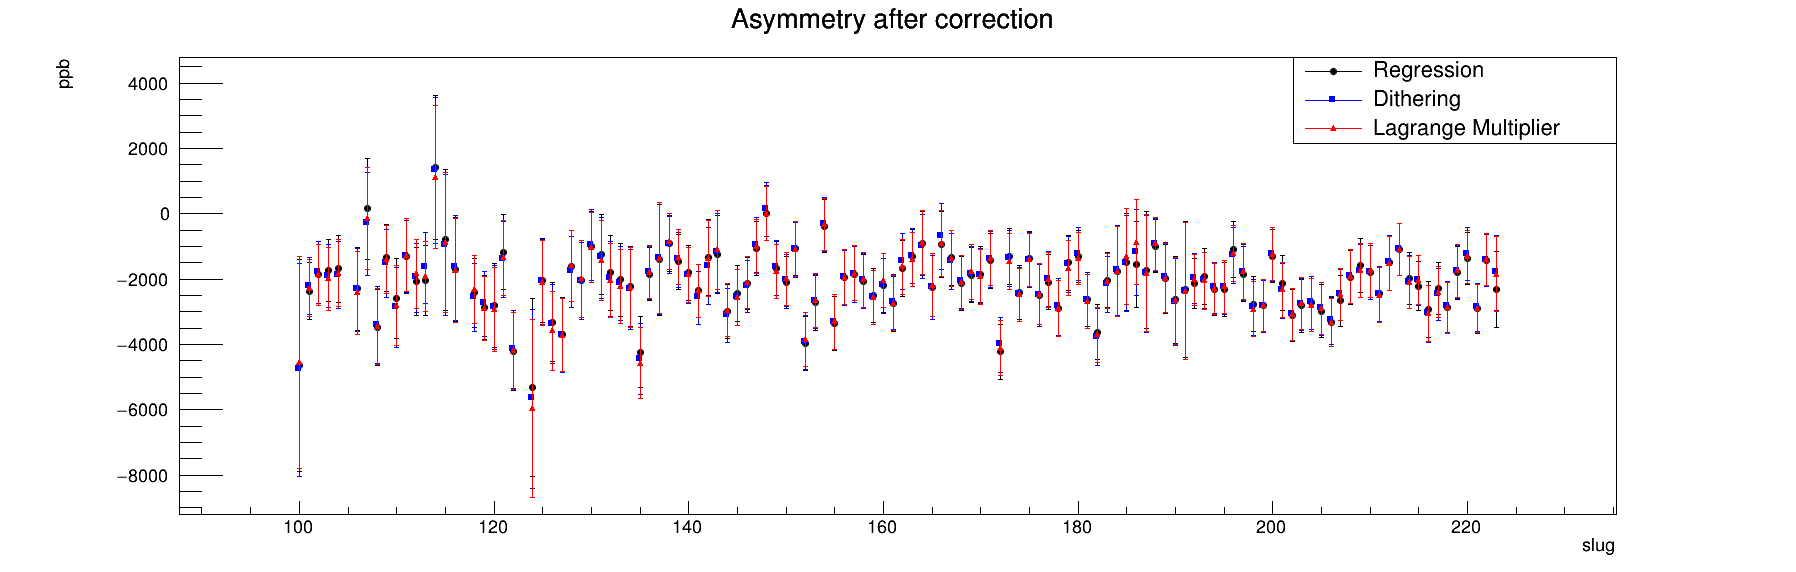
\includegraphics[width=\linewidth]{crex_corrected_asym}
    \caption{Comparison of corrected asymmetries with different methods.}
    \label{fig:crex_corrected_asym}
\end{figure}

%%%%%%%%%%%%%%%%%%%%%%%%%%%%%%%%%%%%%%%%%%%%%%%%%%%%%%%%%%%%%%%%%%%%%%%%
\section{Result}
As we said before, the slow control of IHWP and Wien Filter allow us to check
the possible systematic bias. A part is defined as all runs with the same IHWP state
and Wien Filter setup in a period. By looking at the part asymmetry, we find that 
corrected asymmetries measured with opposite IHWP or Wien Filter state overlap
with each other with $1\sigma$ uncertainty, verifying the unbiasedness of our
measurement.

The pitt plot in Fig.~\ref{fig:crex_part_pitt} shows the asymmetry distribution
for each pitt. The concept of pitt originated from Mark Pitt. The idea is to combine
nearby slugs of alternating IHWP states to have the same (similar) number of events for 
opposite IHWP states. Every pitt includes about 4 slugs, the detailed range definition
of pitt can be found in Cameron's thesis.

%%%%%%%%%%%%%%%%%%%%%%%%
\subsubsection{Pitt and Part Plot}
\begin{figure}
    % comparison of asymmetry from largest time scale to smallest time scale:
    % wien, pitt, slug, run
    \centering
    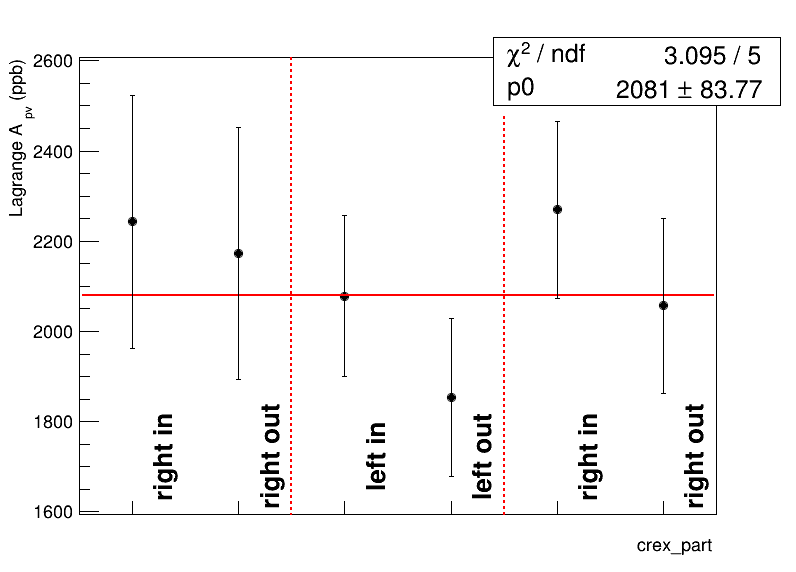
\includegraphics[width=0.49\linewidth]{crex_part_eigen_lagr_asym_main_det_1}
    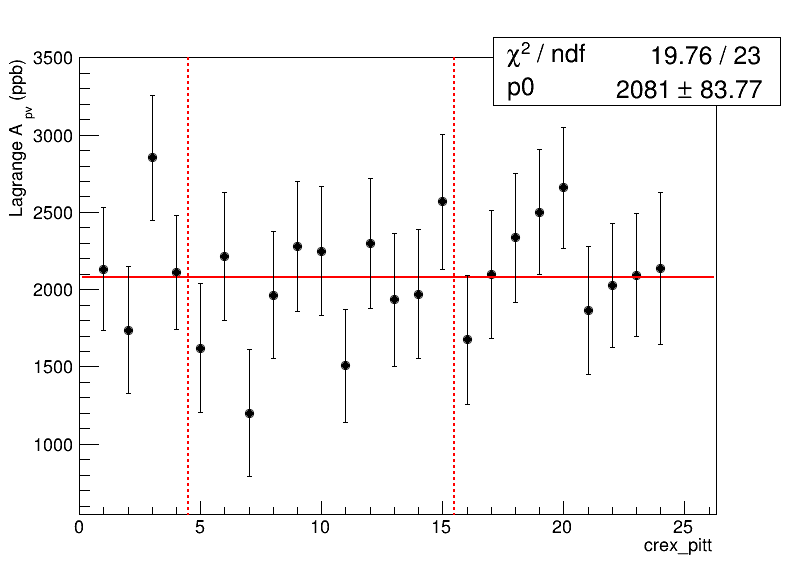
\includegraphics[width=0.49\linewidth]{crex_pitt_eigen_lagr_asym_main_det_1}
    \caption{Part and pitt plot of asymmetry corrected with Lagrange Multiplier.}
    \label{fig:crex_part_pitt}
\end{figure}

From the pitt plot, we read the final corrected asymmetry as $2081 \pm 83.77\ ppb$ (blinded).
The number used in our published result was $2080 \pm 83.77$. The difference 
lies in the 2 miniruns I discard in Table~\ref{tab:short_miniruns} with too small
samples.
